%&preformat-disser
\RequirePackage[l2tabu,orthodox]{nag} % Раскомментировав, можно в логе получать рекомендации относительно правильного использования пакетов и предупреждения об устаревших и нерекомендуемых пакетах
% Формат А4, 14pt (ГОСТ Р 7.0.11-2011, 5.3.6)
\documentclass[a4paper,14pt,oneside,openany]{memoir}

\input{common/setup}               % общие настройки шаблона
\input{common/packages}  % Пакеты общие для диссертации и автореферата
\input{Dissertation/dispackages}         % Пакеты для диссертации
\input{Dissertation/userpackages}        % Пакеты для специфических пользовательских задач

\input{Dissertation/setup}               % Упрощённые настройки шаблона

\input{Dissertation/preamblenames}       % Переопределение именований, чтобы можно было и в преамбуле использовать
\input{common/newnames}  % Новые переменные, которые могут использоваться во всём проекте

%%% Основные сведения %%%
\newcommand{\thesisAuthor}             % Диссертация, ФИО автора
{%
    \texorpdfstring{% \texorpdfstring takes two arguments and uses the first for (La)TeX and the second for pdf
        Ульянов Данила Ярославович % так будет отображаться на титульном листе или в тексте, где будет использоваться переменная
    }{%
        Ульянов, Данила Ярославович% эта запись для свойств pdf-файла. В таком виде, если pdf будет обработан программами для сбора библиографических сведений, будет правильно представлена фамилия.
    }%
}
\newcommand{\thesisAuthorShort}        % Диссертация, ФИО автора инициалами
{\todo{И.О.~Фамилия}}

%\newcommand{\thesisUdk}                % Диссертация, УДК
%{\todo{xxx.xxx}}
\newcommand{\thesisTitle}              % Диссертация, название
{\texorpdfstring{\todo{\MakeUppercase{Название диссертационной работы}}}{Название диссертационной работы}}
\newcommand{\thesisSpecialtyNumber}    % Диссертация, специальность, номер
{\texorpdfstring{\todo{XX.XX.XX}}{XX.XX.XX}}
\newcommand{\thesisSpecialtyTitle}     % Диссертация, специальность, название
{\texorpdfstring{\todo{Название специальности}}{Название специальности}}
\newcommand{\thesisDegree}             % Диссертация, ученая степень
{\todo{кандидата физико-математических наук}}
\newcommand{\thesisDegreeShort}        % Диссертация, ученая степень, краткая запись
{\todo{канд. физ.-мат. наук}}
\newcommand{\thesisCity}               % Диссертация, город написания диссертации
{Нижний Новгород}
\newcommand{\thesisYear}               % Диссертация, год написания диссертации
{\todo{20XX}}
\newcommand{\thesisOrganization}       % Диссертация, организация
{Нижегородский государственный университет им. Н.И.~Лобачевского}
\newcommand{\thesisOrganizationShort}  % Диссертация, краткое название организации для доклада
{ННГУ}

\newcommand{\thesisInOrganization}     % Диссертация, организация в предложном падеже: Работа выполнена в ...
{\todo{учреждении, в~котором выполнялась данная диссертационная работа}}

\newcommand{\supervisorFio}            % Научный руководитель, ФИО
{Турлапов Вадим Евгеньевич}
\newcommand{\supervisorRegalia}        % Научный руководитель, регалии
{\todo{уч. степень, уч. звание}}
\newcommand{\supervisorFioShort}       % Научный руководитель, ФИО
{В.Е.~Турлапов}
\newcommand{\supervisorRegaliaShort}   % Научный руководитель, регалии
{\todo{уч.~ст.,~уч.~зв.}}


\newcommand{\opponentOneFio}           % Оппонент 1, ФИО
{\todo{Фамилия Имя Отчество}}
\newcommand{\opponentOneRegalia}       % Оппонент 1, регалии
{\todo{доктор физико-математических наук, профессор}}
\newcommand{\opponentOneJobPlace}      % Оппонент 1, место работы
{\todo{Не очень длинное название для места работы}}
\newcommand{\opponentOneJobPost}       % Оппонент 1, должность
{\todo{старший научный сотрудник}}

\newcommand{\opponentTwoFio}           % Оппонент 2, ФИО
{\todo{Фамилия Имя Отчество}}
\newcommand{\opponentTwoRegalia}       % Оппонент 2, регалии
{\todo{кандидат физико-математических наук}}
\newcommand{\opponentTwoJobPlace}      % Оппонент 2, место работы
{\todo{Основное место работы c длинным длинным длинным длинным названием}}
\newcommand{\opponentTwoJobPost}       % Оппонент 2, должность
{\todo{старший научный сотрудник}}

\newcommand{\leadingOrganizationTitle} % Ведущая организация, дополнительные строки
{\todo{Федеральное государственное бюджетное образовательное учреждение высшего профессионального образования с~длинным длинным длинным длинным названием}}

\newcommand{\defenseDate}              % Защита, дата
{\todo{DD mmmmmmmm YYYY~г.~в~XX часов}}
\newcommand{\defenseCouncilNumber}     % Защита, номер диссертационного совета
{\todo{Д\,123.456.78}}
\newcommand{\defenseCouncilTitle}      % Защита, учреждение диссертационного совета
{\todo{Название учреждения}}
\newcommand{\defenseCouncilAddress}    % Защита, адрес учреждение диссертационного совета
{\todo{Адрес}}
\newcommand{\defenseCouncilPhone}      % Телефон для справок
{\todo{+7~(0000)~00-00-00}}

\newcommand{\defenseSecretaryFio}      % Секретарь диссертационного совета, ФИО
{\todo{Фамилия Имя Отчество}}
\newcommand{\defenseSecretaryRegalia}  % Секретарь диссертационного совета, регалии
{\todo{д-р~физ.-мат. наук}}            % Для сокращений есть ГОСТы, например: ГОСТ Р 7.0.12-2011 + http://base.garant.ru/179724/#block_30000

\newcommand{\synopsisLibrary}          % Автореферат, название библиотеки
{\todo{Название библиотеки}}
\newcommand{\synopsisDate}             % Автореферат, дата рассылки
{\todo{DD mmmmmmmm YYYY года}}

% To avoid conflict with beamer class use \providecommand
\providecommand{\keywords}%            % Ключевые слова для метаданных PDF диссертации и автореферата
{}      % Основные сведения
\input{common/styles}    % Стили общие для диссертации и автореферата
\input{Dissertation/disstyles}           % Стили для диссертации
\input{Dissertation/userstyles}          % Стили для специфических пользовательских задач
\input{biblio/bibliopreamble}% Настройки библиографии из внешнего файла (там же выбор: встроенная или на основе biblatex)

\input{Dissertation/inclusioncontrol}    % Управление компиляцией отдельных частей диссертации

\begin{document}

\input{common/renames}                   % Переопределение именований

% Структура диссертации (ГОСТ Р 7.0.11-2011, 4)
\include{Dissertation/title}           % Титульный лист
\include{Dissertation/contents}        % Оглавление
\include{Dissertation/introduction}    % Введение
\chapter{Обзор публикаций и программного обеспечения по теме исследования} \label{chapt1}

\section{Твердотельное моделирование} \label{solid_modeling}

В геометрическом моделировании используются термины «поверхностное моделирование» (моделирование поверхностей) и «твердотельное моделирование» (моделирование твердых тел, solid modelling). В первом случае результатом моделирования является некоторая оболочка (или несколько оболочек), описывающая поверхность моделируемого объекта. Во втором случае результатом моделирования является полная геометрическая модель твердого тела, которая позволяет автоматизированно ответить на любой вопрос о его геометрических свойствах (вычисление объема тела, поиск пересечений с другими телами, изображение тела с любого ракурса и т.д.). Процесс моделирования в первом случае также значительно отличается от процесса моделирования во втором случае.

В поверхностном моделировании сначала создаются и модифицируются требуемым образом поверхности, описывающие отдельные элементы моделируемого объекта. Эти поверхности обрезают по линиям пересечения, сопрягают друг с другом поверхностями скругления или перехода (fillets, chamfers), а также выполняют над ними другие операции. Затем из полученных поверхностей собирают оболочку. Этот подход к моделированию является непосредственной эволюцией традиционного подхода к построению чертежей. В поверхностном моделировании результирующая оболочка не обязательно должна быть замкнутой. Она может отражать лишь часть (главную часть) моделируемого объекта. Поверхностное моделирование позволяет сосредоточить усилия на сложных формах объекта и широко применяется для проектирования кузовов автомобилей и планеров самолетов.

В твердотельном моделировании с самого начала работа идет с целостной моделью тела, а не с отдельными поверхностями. Например, в граничном представлении, оболочки (shells) полностью описывают поверхности моделируемых объектов, отделяющие их внутренний объем от остальной части пространства. Процесс построения тела в данном случае часто аналогичен процессу изготовления моделируемого объекта. Сначала создается модель некоторой заготовки простой формы. Далее заготовка изменяется необходимым образом. Для этого могут используются булевы операции над телами, операция построения тонкостенного тела из заготовки, операция скругления ребер, операция построения ребер жесткости и другие операции. На практике используется несколько представлений геометрии "--- подходов к описанию твердых тел.

Понятие твердотельного моделирования опирается на потребность в информационной полноте в системах механического геометрического моделирования в том смысле, что любая компьютерная модель должна отвечать на все геометрические вопросы, которые могут быть заданы по отношению к соответствующему физическому объекту. Это требование не противоречит возможности существования нескольких компьютерных представлений одного и того же физического объекта, если такие представления согласованы. Невозможно вычислительно проверить информационную полноту представления, если понятие физического объекта не определено в терминах вычислимых математических свойств и не зависит от какого-либо конкретного представления. Такие рассуждения привели к разработке парадигмы моделирования, которая сформировала область твердотельного моделирования, как мы ее знаем сегодня.

Любая схема представления геометрия является методом хранения информации о классе полу-аналитических подмножеств евклидова пространства. Это означает, что все представления представляют собой разные способы организации одних и тех же геометрических и топологических данных в форме структур данных. Однако, моделируемое пространство каждого отдельно взятого представления геометрии ограничено, и ни одна схема представления геометрии не может представить все возможные твердые тела. Например, тела представленные граничным представлением (Boundary representation) не всегда могут быть представлены телом движения (sweep solid), кроме простейших случаев. Это заставляет современные системы геометрического моделирования поддерживать несколько схем представления твердых тел, а также способствовать эффективному преобразованию схем представления.

Обзор основных представлений твердотельной геометрии дан \cite{Requicha80} ещё в 1980 году. Там же приведён перечень формальных свойств (таких как уникальность, однозначность и т.п.) систем представления твердых тел, а так же понятие R-множеств и регуляризованных операций над множествами. Однако, поиск оптимальных представлений для конкретных задач и исследование гибридных схем продолжаются и по сей день.

Ниже приведён обзор основных подходов к представлению твердых тел.

\section{Порождение параметризованных примитивов} \label{sect_primitive_instatiation}

Один из первых подходов к представлению твердых тел возник в области производства, главным образом в контексте так называемой Group Technology \cite{Gall73}. Он основан на понятии семейств объектов, при этом каждый член семейства отличается от других уникальным набором параметров. Каждое семейство иначе может быть названо \textit{обобщенным примитивом}, отдельные объекты в семействе называются \textit{экземплярами примитива}. Экземпляры примитивов задаются конечным набором параметров.

Отличительной характеристикой чистого подхода порождения примитивов, является отсутствие средств комбинирования примитивов для создания новых, более сложных объектов.

Такая схема представления твердотельной геометрии удобна и проста в использовании, но только до тех пор пока набор обобщённых примитивов и их параметров достаточно мал. Другим недостатком представления является сложность построения алгоритмов для вычисления свойств представляемых тел. Каждое семейство примитивов приходится обрабатывать как специальный случай, что не позволяет единообразно обрабатывать геометрию.

\section{Карта заполнения пространства} \label{sect_spatial_occupancy_enum}

Представление тела в виде \textit{карты заполнения пространства} (Spatial Occupancy Enumeration), более известное, в настоящее время, как \textit{воксельное} представление, представляет из себя список пространственных ячеек, занимаемых телом. Эти ячейки, также называемые вокселями, обычно являются параллелепипедами фиксированного размера и лежат в фиксированной пространственной сетке. В такой системе, каждая ячейка может быть представлена координатами единственной точки, например центроидом ячейки. Обычно подразумевается также определённый порядок обхода сетки. Соответствующие упорядоченные наборы ячеек называют \textit{пространственными массивами} (\textit{spatial arrays}).

Пространственные массивы, как правило, слишком подробны (избыточны) в качестве основного представления для моделирования однородных твердых тел с требуемой точностью. Однако алгоритмы и структуры данных, используемые для них, могут быть существенно проще.

Подробность воксельного представления может быть скомпенсирована правильно выбранной иерархической структурой данных (за счет пропуска пустого и/или однородного пространства) ценой усложнения алгоритмов обработки данных. Уже в работе \cite{REDD78} предлагалось строить дерево адаптивных разбиений пространства для уменьшения объема хранимых данных. Позже в работе \cite{Meagher82} было предложено понятие восьмеричного дерева (октодерево, octree) в качестве эффективной структуры для хранения и обработки воксельных данных. С тех пор октодеревья получили широкое распространение. Часто воксельное представление используется как вспомогательное, для работы с другим представлением. Дальнейшие исследования предлагали множество вариантов развития этой структуры. Дополненные октодеревья предложенные в работе [8] добавляют набор специальных узлов для представления плоских граней, ребер и вершин. В работе [16] предлагается использовать фрагменты описания CSG деревьев (см. раздел \ref{sect_csg}) в узлах октодерева, для последующей реконструкции модели. Первый подход оптимизирован для совместного использования воксельного и граничного (см. раздел \ref{sect_boundary_rep}) представления и позволяет легче переходить от одного к другому. В то же время второй подход рассчитан на совместное использование воксельного и CSG представления. Ещё одним вариантом гибридного подхода являются адаптивно заданные поля расстояний (Adaptively sampled distance fields), описанные в работах [17, 13]. Такой подход, совмещающий функциональное (см. раздел \ref{sect_implicit}) и воксельное представления, используется как внутреннее представление, например, для инструментов цифрового скульптинга (англ. sculpting-style design tools) \todo{[43]} и моделирования машинной обработки (англ. machining simulations) \todo{[46]}.

D. Meagher, “Geometric modeling using octree encoding,” Computer Graphics
and Image Processing, vol. 19, no. 2, pp. 129–147, June 1982.

[8] P. Brunet and I. Navazo, Solid representation and operation using extended
octrees," ACM Trans. Graph., vol. 9, no. 2, pp. 170{197, Apr. 1990. [Online].
Available: http://doi.acm.org/10.1145/78956.78959

[16] E. Dyllong and C. Grimm, A reliable extended octree representation of
csg objects with an adaptive subdivision depth," in Parallel Processing and
Applied Mathematics, ser. Lecture Notes in Computer Science, R. Wyrzykowski,
J. Dongarra, K. Karczewski, and J. Wasniewski, Eds. Springer Berlin
Heidelberg, 2008, vol. 4967, pp. 1341{1350. [Online]. Available: http:
//dx.doi.org/10.1007/978-3-540-68111-3 142

[17] S. F. Frisken, R. N. Perry, A. P. Rockwood, and T. R. Jones, Adaptively
sampled distance fields: a general representation of shape for computer
graphics," in Proceedings of the 27th annual conference on Computer graphics
and interactive techniques, ser. SIGGRAPH ’00. New York, NY, USA: ACM
Press/Addison-Wesley Publishing Co., 2000, pp. 249{254. [Online]. Available:
http://dx.doi.org/10.1145/344779.344899

[13] L. de Figueiredo, L. Velho, and J. de Oliveira, Revisiting adaptively sampled
distance fields," in Computer Graphics and Image Processing, 2001 Proceedings
of XIV Brazilian Symposium on, 2001, pp. 377

[43] R. N. Perry and S. F. Frisken, Kizamu: a system for sculpting digital
characters," in Proceedings of the 28th annual conference on Computer graphics
and interactive techniques, ser. SIGGRAPH ’01. New York, NY, USA: ACM,
2001, pp. 47{56. [Online]. Available: http://doi.acm.org/10.1145/383259.383264

[46] A. Sullivan, H. Erdim, R. N. Perry, and S. F. Frisken, High accuracy
nc milling simulation using composite adaptively sampled distance fields,"
Comput. Aided Des., vol. 44, no. 6, pp. 522{536, Jun. 2012. [Online]. Available:
http://dx.doi.org/10.1016/j.cad.2012.02.002

\section{{Декомпозиция на ячейки} \label{sect_cell_decompositions}

Твердое тело может быть представлено разложением на набор ячеек. Схемы воксельного представления являются частными случаями разложения на ячейки, где все ячейки представленны параллелепипедами и образуют регулярную сетку. Более подробное определение дано в \cite{Requicha80}.

Наиболее распространенным частным случаем декомпозиции на ячейки является триангуляция. Сплошная триангуляция плоскогранного тела представляет из себя разложение тела на составляющие тетраэдры, которые должны быть непересекающимися, либо иметь ровно одну общую грань, либо ребро, либо вершину. Тело с криволинейной поверхностью, в принципе, таким же образом может быть триангулированно с разложением на криволинейные тетраэдры, однако такой вариант в настоящее время практически не используется из-за повышенной сложности создания и обработки геометрии.

Представление тела в виде сплошной триангуляции используется, в основном, для расчетов методом конечных элементов, для численного решения уравнений в частных производных.

В работе \cite{A combined octree/Delaunay method for fully automatic 3-d mesh generation} 1990 был предложен полностью автоматический метод построения сплошной триангуляции для твердого тела с использованием окто-дерева и триангуляции Делоне.

В работе \cite{Modeling with Simplicial Complexes} 1996 топологическая концепция симплициального комплекса ставится в соответствие триангуляции для твердотельного моделирования. 

\section{Заметание} \label{sect_sweeping}

Множество точек движущееся через пространство заметает определённый объем (тело), который может быть однозначно задан движущимся множеством точек и траекторией. Такое представление важно, например, для определения части материала, удаляемого фрезой при производстве, по мере её перемещения по заданной траектории. Большинство коммерческих САПР предоставляют ограниченные функциональные возможности для создания тел заметания. Как правило, используется формирование тела заметания перемещением или вращением замкнутой плоской фигуры. В первом случае процесс формирования называется заметанием при трансляции (translational sweeping), во втором случае "--- построением фигуры вращения (swinging, rotational sweeping).

\section{Граничные представления} \label{sect_boundary_rep}

Граничное представление для твердотельной геометрии было впервые представлено в работе [1] в 1974 году, что повлекло за собой обширные исследования структур данных для САПР во второй половине 1970-х и 1980-х годов.

[1] Braid, I.C., Designing with volumes, Ph.D. Thesis, Cambridge University, England, (1974).

В этой схеме твердое тело представлено с помощью задания его границы из элементов различных поверхностей. Так как граница твердого тела должна быть замкнута, каждая точка в пространстве однозначно может быть классифицирована как находящаяся внутри или снаружи тела. Используя технику бросания луча, можно подсчитать количество пересечений  луча с границей твердого тела. Четное число пересечений соответствует внешним точкам, а нечетное "--- внутренним. Корректное граничное представление твердого тела также должно удовлетворять следующим условиям: все пары вершин не совпадают, пары ребер либо не пересекаются, либо пересекаются в одной вершине, а пары граней не пересекаются или пересекаются на общем ребре либо в общей вершине. Для хранения граничных представлений твердых тел были разработаны несколько структур данных, представляющих собой комбинаторные карты. В дополнение к плоскостным граням современные системы, использующие граничное представление, обеспечивают поддержку поверхностей второго порядка и NURBS поверхностей. Граничные представления стали доминирующей схемой представления твердых тел в большинстве коммерческих систем из-за их гибкости и универсальности. Популярности граничных представлений также способствовала сравнительная простота визуализации модели. При массовом распространении аппаратных средств визуализации триангулированных поверхностей (графические процессоры, англ. Graphic Processing Unit, GPU) это преимущество стало одним из решающих. Однако, у граничных представлений есть и недостатки. Создать корректное граничное представление твердого тела не простая задача. Еще сложнее поддерживать представление корректным при редактировании модели. Об этом свидетельствует, например, разнообразие существующих инструментов для устранения типичных проблем, возникающих в результате работы с триангулированными сетками [27, 32].

[27] J. LaMarche. Prepping blender files for 3d printing. [Online]. Available:
http://www.shapeways.com/tutorials/prepping blender files for 3d printing

[32] Meshlab Stuff. On the subtle art of mesh cleaning. [Online]. Available: http:
//meshlabstuff.blogspot.com/2009/03/on-subtle-art-of-mesh-cleaning.html

Связанный недостаток "--- сложность. Разработка надежного конкурентоспособного геометрического ядра, основанного на граничных представлениях, сейчас требует ресурсов крупной международной компании. В основе таких систем часто лежат различные задачи глобальной оптимизации, а так же алгоритмы пересечения и разбиения NURBS, что приводит к проблемам связанным с производительностью алгоритмов и точностью чисел с плавающей точкой.

\section{Функциональное представление} \label{sect_implicit}

Понятие функционального представления (F-rep, implicit modeling) приводится в \todo{"Function representation in geometric modeling: concepts, implementation and applications" [2]} как универсальное представление для тел заданных в многомерном пространстве. Тело, как множество точек в многомерном пространстве, определяется одной непрерывной вещественной функцией координат $f(x_{1},x_{2},...,x_{n})$. Эта функция вычисляется в данной точке путем обхода древовидной структуры с функциями-примитивами во внешних узлах и функциями-операциями во внутренних. Точки, для которых выполняется $f(x_{1},x_{2},...,x_{n})\geq 0$ принадлежат телу, точки, для которых $ f(x_{1},x_{2},...,x_{n})<0$ находятся вне тела. Множество точек, для которых $f(x_{1},x_{2},...,x_{n})=0$ составляет границу тела. Поверхность, состоящая из множества точек, соответствующих определённому значению функции называется изоповерхностью. Так в трехмерном пространстве, простейшей формой предиката является условие знака вещественной функции, приводящее к представлению множеств по равенствам и неравенствам. Например, если $ f = ax + by + cz + d$  условия $f (p) = 0$, $f (p)> 0$ и $f (p) <0$ представляют соответственно плоскость и два открытых линейных полупространства. Более сложные функциональные примитивы могут быть определены с помощью булевых комбинаций более простых предикатов.

Первым применением функционального подхода к моделированию сложных тел можно считать R-функции Рвачева [63, 74]. Этот подход позволяющий представить твердое тело в виде единственной вещественной функции использовался для задач физического моделирования. Были разработаны подходы для применения теоретико-множественных операций над телами и способы обхода $C^1$ прерывности функций, представляющих твердые тела.

Functional representations have several advantages over boundary representations.
F-reps also have arbitrarily high resolution, as the expression can be evaluated at as many
points as desired. Finally, there exists an efficient rendering strategy based on spatial
subdivision which dovetails with ASDF creation and population.

Функциональное представление может быть тривиально преобразовано в воксельное представление путем вычисления значений в узлах воксельной сетки, а также в граничное представление с использованием алгоритмов триангуляции, например, алгоритма марширующих кубов [29] или марширующих тетраэдров [36].

[29] W. E. Lorensen and H. E. Cline, Marching cubes: A high resolution 3d surface
construction algorithm," SIGGRAPH Comput. Graph., vol. 21, no. 4, pp. 163{
169, Aug. 1987. [Online]. Available: http://doi.acm.org/10.1145/37402.37422

36 H. Muller and M. Wehle, Visualization of implicit surfaces using adaptive tetrahedrizations," Scientific Visualization Conference, vol. 0, p. 243, 1997.

\section{Конструктивная блочная геометрия} \label{sect_csg}

Конструктивная блочная геометрия (Constructive Solid Geometry или CSG) представляет собой семейство схем для представления твердых тел в виде булевых комбинаций примитивов с помощью регуляризованных \cite{Requicha80} \cite{Requicha77} операций на множествах. CSG представления имеют форму упорядоченных двоичных деревьев, где нетерминальные (внутренние) узлы представляют собой либо твердотельные преобразования (перенос и поворот), либо регуляризованные операции на множествах. Терминальные (листовые) узлы являются примитивами, представляющими замкнутые регулярные множества. Таким образом, каждое поддерево представляет собой множество, полученное в результате применения указанных операций на множестве, представленном листовыми примитивами поддерева. Привлекательные свойства CSG включают в себя компактность, гарантированную корректность твердых тел (при использовании корректных твердых тел в качестве примитивов), и естественный контроль формы твердого тела в терминах параметров высокого уровня, определяющих примитивы твердого тела, их положения и ориентации. Относительно простая структура данных и изящные рекурсивные алгоритмы еще больше способствовали популярности CSG на заре развития САПР и геометрического моделирования. Позже, проблемы CSG подхода как основного представления твердых тел всё же перевесили его преимущества. К таким проблемам относят: сложность прямой визуализации CSG объектов (без перехода к граничному представлению), сложность перехода к граничному представлению, сложность задания незамкнутых объектов (это возможно если использовать незамкнутые примитивы, но тогда необходимо отказаться от одного из главных преимуществ — гарантированной корректности) и т. д.

Сейчас CSG представление используется в основном как вспомогательное или промежуточное представление, для выполнения булевых операций над телами. В то же время, для многих задач CSG представление остается наиболее естественным. В таких задачах, отказ от дополнительных схем представления позволил бы значительно упростить соответствующие САПР, повысить быстродействие систем. Настоящая работа призвана устранить один из главных недостатков CSG представления: невозможность интерактивной визуализации сложных CSG моделей, и тем самым способствовать развитию САПР использующих CSG как основное представление твердых тел.

\section{Подходы к визуализации CSG} \label{sect_csg_vis}

Самым ранним способом визуализации CSG моделей была отрисовка линиями (wireframe). Для этого необходимо построить линии пересечения всех поверхностей в модели и спроектировать их на экранную плоскость. Позже, этот метод начали дополнять удалением невидимых линий. [e.g. Appel67], [An algorithm for eliminating the hidden lines in computer-drawn polyhedra 68]

Идея применения трассировки лучей (ray casting) для визуализации CSG моделей, по видимому, ваервые была опубликована в работе \todo{Goldstein and Nagel}. В этой работе трассировка лучей применяется для получения затененных изображений твердотельных моделей. Чтобы получить такое изображение авторы моделировали процесс, обратный получению фотографии. Для каждого пикселя изображения, строится луч и определяется его пересечение с виртуальной сценой. Ближайшее к наблюдателю пересечение луча с поверхностью определяет видимую поверхность. Вычислив нормаль к поверхности в точке пересечения и зная положение источника света, можно рассчитать яркость каждого пикселя. 

В работе формулируется основная идея алгоритма пересечения луча и CSG модели. Каждая точка пересечения луча и геометрии (в порядке от ближних к дальним) анализируется на принадлежность логическому выражению, соответствующему части модели -- региону. На основе этого метода была разработана коммерческая CAD/CAM система SynthaVision, которая позволяла получать затененные изображения твердотельных моделей.

Многие эксперты в CAD/CAM области того времени считали трассировку лучей непрактичным методом "грубой силы" \todo{[Roth]}. \todo{[Roth]} в своей работе приводит практическое описание алгоритма трассировки лучей для задачи визуализации CSG моделей, а также приводит оптимизации алгоритма. \todo{[Roth]} использует ограничивающие объемы для ускоренного отбрасывания CSG поддеревьев, гарантированно непересекающихся с лучом. \todo{[Roth]} делает вывод о важности пространственной когерентности примитивов в дереве и предполагает, что CSG дерево может быть автоматически переупорядочено для улучшения пространственной когерентности. Дальнейшие оптимизации для алгоритма трассировки лучей применительно к CSG были предложены в работе \todo{[Bronsvoort84]}.

Алгоритмы бросания лучей \todo{[Roth, Goldstein and Malin]} применяют один и тот же алгоритм 
Алгоритмы бросания (англ. ray-firing, ray-shooting) лучей \todo{[Roth, Goldstein and Malin]} применяют один и тот же алгоритм для каждой точки на экране для определения видимости поверхностей. Задача поиска поверхности соответствующей CSG выражению сводится к одномерной задаче на луче. Формализованная классификация одномерных алгоритмов решения булевых выражений дана в работе \todo{[Tilove(atheron-15)]}. Главным преимуществом подходов, основанных на бросании лучей, является отсутствие необходимости вычислять полную граничную поверхность, соответствующую CSG модели. Для определения видимой точки на луче, пересекающем CSG модель, можно использовать следующий алгоритм:

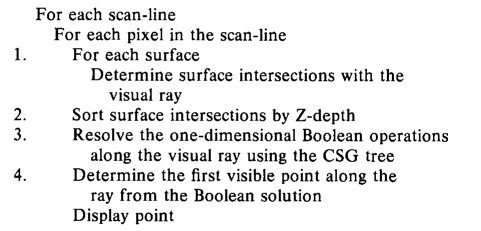
\includegraphics[]{1.png}

\todo{Рисунок 3} иллюстрирует вычисление булевых операций в одномерном пространстве для двух примитивов. В дополнение к простоте, метод имеет дополнительное преимущество для визуализации: после того как ближайшая точка определена, дальнейшие вычисления можно отбросить. Однако, перед тем как применить эти простые правила, необходимо пересечь луч с CSG примитивами и отсортировать точки пересечения. К тому же, все эти шаги должны быть выполнены для каждого пикселя изображения. \todo{[Roth]} описывает процедуру отсечения для уменьшения числа поверхностей, с которыми нужно пересечь луч для каждого пикселя. Однако, хотя такая оптимизация и дает эффект, тем не менее вычислительная сложность алгоритма не меняется. \todo{[Roth]} также приводит метод для определения и визуализации только силуэта и линий пересечения поверхностей, но этот метод не совместим с затененной визуализацией.

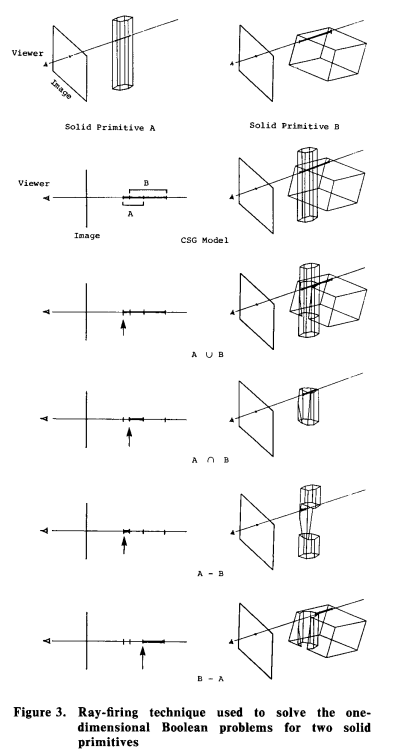
\includegraphics[]{2.png}}

Широко используемый в то время (1980-е) для задачи определения видимости полигонов, построчный подход к визуализации (англ. scanline rendering), также был адаптирован для визуализации CSG моделей \todo{[atherton1983]}. Типичный scanline алгоритм, использующий Y-X-Z сортировку полигонов, представлен ниже:

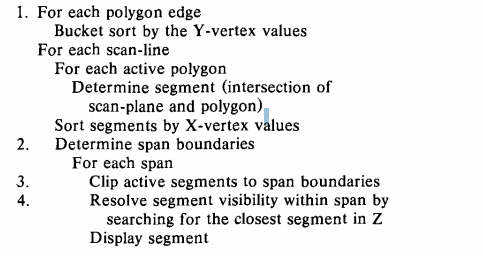
\includegraphics[]{scanline.png}}

Сегментом в scanline алгоритмах называется часть полигона, образованная пересечением scanline плоскости и полигона.

Интервалом называется непрерывная часть scanline, для которой возможно определить видимый сегмент. 

Алгоритм, предложенный \todo{[atherton1983]} использует те же 4 шага, что и обычный алгоритм scanline, однако вместо определения видимости сегмента в интервале по его близости к виртуальной камере (наблюдателю), используется более сложная процедура, аналогичная процедуре поиска видимой поверхности с помощью трассировки луча, примененной к концам интервала. В случае, если для концов интервала видимыми становятся разные поверхности, интервал рекурсивно разбивается.

Как и во многих других исследованиях, посвещенных scanline алгоритмам, в работе \todo{[atherton1983]} была предпринята попытка использовать свойства когерентности геометрии для оптимизации вычислений. Когерентность интервалов можно считать первым улучшением по сравнению с трассировкой лучей. Если на границах интервала видима одна и та же поверхность, то и результаты расчета затенения можно интерполировать между концами интервала.

Все разнообразие алгоритмов визуализации CSG моделей можно разделить на три базовых подхода. Первый подход основан на предварительном расчете полной границы CSG объекта (переход к граничному представлению), которая затем тесселируется и визуализируется с использованием традиционных инструментов 3D графики (Direct3D, OpenGL). Поскольку расчет границы является  вычислительно трудоемкой операцией, алгоритмы данной группы зачастую применимы только для статических сцен и не позволяют выполнять интерактивное редактирование конструктивных моделей.

Второй подход основан на переходе к воксельному представлению, для этого достаточно иметь возможность классифицировать точку относительно CSG дерева. После этого геометрию можно визуализировать как 3Д текстуру, средствами объемного рендеринга (англ. volume rendering). К недостатком такого подхода можно отнести большой объем занимаемого пространства и ограниченную точность представления (шагом воксельной сетки). Однако такой подход достаточно прост и производительность визуализации не зависит от сложности CSG дерева. \todo{Hardware-based slicing algorithm for CSG [58, 44]}.

Третий подход построен на базе техник анализа изображения (англ. image-based), которые генерируют только изображение CSG модели с заданного ракурса, избегая трудоемких вычислений полной границы. Большинство таких методов разработано для графической аппаратуры и реализуется с помощью многопроходных и зависящих от ракурса техник, интенсивно использующих буферы глубины и трафарета. В рамках данного подхода широкое распространение получили алгоритм \todo{Goldfeather [1, 2]} и алгоритм последовательного вычитания выпуклых оболочек (англ. Sequenced Convex Subtraction, SCS) \todo{[3]}. Первый из них поддерживает любые CSG примитивы, в то время как второй применим только к сценам, состоящим из выпуклых примитивов. При этом ни один из указанных  алгоритмов не позволяет визуализировать конструктивные модели напрямую. Вместо этого, CSG выражение должно быть преобразовано в дизъюнктивную нормальную форму (дизъюнкция с минимальным числом элементарных конъюнкций), что может приводить к экспоненциальному росту размера булевой формулы, значительно ограничивая  масштабируемость и производительность алгоритмов. Позже был предложен алгоритм Improved Layered Goldfeather Algorithm (General purpose Z-buffer CSG rendering with consumer level hardware). Обзор техник, использующих буфер глубины, представлен в работе \todo{[93]}. Визуализация CSG моделей с использованием двустороннего теста глубины описанная в \todo{[42]} позволила улучшить разложение сцены по слоям, используя аппаратный тест глубины для расчета теней. В работе \todo{[52]} были предложены улучшения SCS алгоритма, закадровый (англ. off-screen) рендеринг, поддерживаемый теперь аппаратно, наряду с запросом видимости OpenGL (для вычисления количества слоев) позволили увеличить производительность метода. 3D-графическая библиотека \todo{OpenCSG [53]} реализует интерактивный рендеринг CSG с использованием таких алгоритмов как Goldfeather и SCS. 

Альтернативный подход был предложен в более поздней работе \cmd{[4]} и получил название Blister. Вместо нормальной формы, данный метод преобразует CSG формулу к списку BList \todo{[5]}, содержащему каждый примитив ровно один раз. Для визуализации заданной конструктивной модели Blister задействует многопроходную технику разложения сцены по слоям (англ. depth peeling), с помощью которой входная сцена разбивается на слои, все фрагменты которых имеют одинаковый индекс близости (занимают равные позиции в списке фрагментов, отсортированных по мере удаления от камеры). Точки каждого слоя классифицируются согласно заданному CSG выражению и комбинируются для синтеза окончательного изображения. Показано, что для модели с $k$ слоями глубины и $n$ примитивами алгоритм вычисляет изображение за время $O(kn)$. В худшем случае $k$ линейно зависит от $n$, поэтому трудоемкость следует оценить как $O(n^2)$.

Указанные выше алгоритмы обеспечивают интерактивное отображение конструктивных моделей малой или средней  сложности (от нескольких сотен до нескольких десятков тысяч примитивов). При этом их общей чертой является активное использование многопроходных схем, которые ставят скорость рендеринга в зависимость от пропускной способности памяти. На протяжении последних десяти лет пропускная способность памяти GPU растет значительно медленнее производительности вычислительных модулей,  что делает передачу данных узким местом во многих GPU алгоритмах.

Альтернативный подход к визуализации конструктивных сцен был предложен в работе [6], где была предпринята попытка распределения вычислений между центральным и графическим процессором. Для этого входное CSG дерево декомпозируется на простые составляющие (содержащие малое число примитивов), которые затем визуализируются на GPU методом трассировки лучей. Входной CSG объект разбивается до тех пор, пока отдельные его части не будут соответствовать одиночным CSG примитивам или булевой  комбинации двух примитивов. Очевидно, что некоторые фрагменты модели не могут быть разбиты согласно двум указанным случаям (области, содержащие вершины 3-ого и более высоких порядков). Такие фрагменты алгоритмом отбрасываются, что выражается в визуальных артефактах при попытке увеличить изображение на экране монитора. Хотя данный подход оказался эффективным для простых сцен (сотни примитивов), более сложные модели требуют разбиения на большое число простых частей, что ведет к значительному росту числа вызовов отрисовки (англ. draw call) и снижению производительности.

Трассировка лучей для поиска пересечения с целым CSG деревом также возможна и применяется довольно широко. Однако большинство подходов к визуализации CSG сцен требует расчета всех пересечений луча с составляющими объект примитивами. При этом луч разбивается на набор интервалов, соответствующих пересекаемым примитивам. Затем к ним применяются правила булевой алгебры для вычисления ближайшей точки, расположенной на границе конструктивного объекта. Поскольку луч следует пересечь со всеми примитивами сцены, данный алгоритм является крайне вычислительно затратным. Кроме того, он плохо приспособлен для графических процессоров, которые не имеют ресурсов для хранения такого числа интервалов для десятков тысяч лучей. Тем не менее, для относительно простых сцен “интервальная” трассировка лучей на GPU вполне возможна, что наглядно показано в работе \todo{[7]}. В любом случае, данный алгоритм плохо масштабируется с ростом сложности сцены и числа слоев (влияет на число интервалов).

Совершенно другой подход к визуализации CSG моделей  на базе трассировки лучей был представлен в работе \todo{[8]} и основан на поиске ближайших точек соударения лучей с  примитивами 3D сцены. Алгоритм использует концепцию конечного автомата для вычисления точки пересечения с границей CSG модели. При этом требуется, чтобы базовые примитивы были замкнутыми (допустимо обобщение для полупространств, заданных ориентированными поверхностями), имели согласованное поле нормалей и не содержали самопересечений. Элегантность решения и приемлемые ограничения позволяют довольно просто реализовать поддержку конструктивных моделей в любой программной системе, основанной на трассировке лучей. Хотя указанная работа не содержит упоминаний о практических испытаниях алгоритма, он представляется наилучшей основой для разработки специализированной версии для GPU.

\section{Ускоряющие структуры} \label{sect_acceleration_structures}

Для эффективной визуализации многие алгоритмы используют различные структуры данных, которые в контексте визуализации принято называть ускоряющими структурами (англ. acceleration structure). Ускоряющие структуры могут использоваться для пропуска пустого пространства в случае визуализации воксельных представлений. В подходах использующих растеризацию, ускоряющие структуры помогают отсекать невидимую геометрию. Особенно критичны ускоряющие структуры для трассировки лучей. Наиболее трудоемкой операцией в большинстве алгоритмов на базе трассировки лучей является поиск ближайшей точки пересечения луча с объектами сцены. Перед тестированием луча на пересечение с геометрией сцены определяется его пересечение с ускоряющей структурой (данная операция обычно называется «обходом»). В качестве результата ускоряющая структура возвращает ближайшую область пространства с подмножеством примитивов сцены. Процедура трассировки тестирует луч на пересечение с примитивами данного подмножества. Если точка соударения не обнаружена, то ускоряющая структура запрашивается повторно для получения нового подмножества примитивов. Этот процесс продолжается до тех пор, пока для луча не будет найдено соударение или не будет установлено, что данный луч не пересекает сцену.

Расчет точки пересечения луча с объектами сцены относится к задачам поиска, поэтому все ускоряющие структуры реализуют некоторый механизм пространственной сортировки объектов. С точки зрения базового подхода к сортировке все ускоряющие структуры можно разделить на два типа: разбиения пространства (англ. spatial subdivision) и иерархии объектов (англ. object hierarchy). Данные типы являются двойственными по своей природе. Разбиения пространства позволяют уникально представить каждую точку пространства, однако каждый примитив сцены может перекрываться любым числом ячеек. Иерархии объектов позволяют уникально представить каждый примитив, однако каждая точка сцены может перекрываться любым числом ячеек. Примерами разбиений пространства являются такие структуры, как регулярные \todo{[11]} или иерархические \todo{[12]} сетки, октодеревья \todo{[13]} и k-d деревья \todo{[14]}, которые отличаются степенью регулярности \todo{[15]}. Напротив, иерархии ограничивающих объемов \todo{[16]} и их варианты (такие как иерархии ограничивающих интервалов \todo{[17; 18]}) служат примерами иерархий объектов. Развитие методов трассировки лучей неразрывно связано с развитием ускоряющих структур, алгоритмов их построения и обхода. Подробному обзору ускоряющих структур и их относительной эффективности посвящена работа \todo{[19]}.
В большинстве случаев ускоряющие структуры строятся на этапе препроцессирования сцены, поэтому трудоемкость их построения не учитывается на этапе визуализации. Данный подход допустимо применять только для статических сцен (с неизменной геометрией), во время отображения которых возможны перемещения лишь виртуальной камеры и изменения источников света. Для обработки динамических сцен (с подвижной геометрией) необходимо выполнять повторное построение или частичное обновление ускоряющей структуры каждый раз при модификации объектов.           % Глава 1
\chapter{Визуализация моделей конструктивной блочной геометрии} \label{chapt2}

Конструктивная блочная геометрия (англ. Constructive Solid Geometry или CSG) \cite{Requicha80} представляет собой подход к геометрическому моделированию твердых, который сводится к составлению сложных тел из более простых геометрических примитивов. В отличие от подходов поверхностного моделирования, CSG используется для твердотельного моделирования, так как CSG модель задает и поверхность и объем тела.

Настоящая глава определяет модели конструктивной геометрии в терминах \textit{примитивов}, \textit{операций} и \textit{деревьев}. Описаны обход и обработка CSG деревьев. В контексте CSG визуализации, трансформация и симплификация дерева производятся как предварительные шаги, необходимые для последующей эффективной визуализации.

Настоящая глава приводит основные модели и алгоритмы используемые для CSG визуализации, а также описан метод интерактивной фотореалистичной визуализации моделей конструктивно-блочной геометрии предложенный в настоящей работе.

\todo{дописать}

\section{Примитивы} \label{sect_primitives}

Геометрические объекты используемые в CSG моделировании называют \textit{примитивами}. Примитивы определяют свой объем, разделяя пространство на внутреннюю и внешнюю области. Поверхность примитива находится на границе между внутренней и внешней областями.

Набор примитивов доступных в системах CSG моделирования обычно состоит из сфер, эллипсоидов, параллелепипедов, тетраэдров, цилиндров, конусов и торов. Как правило, все примитивы параметризованы. Формально, набор примитивов определяет только типы поверхности, доступные для CSG моделирования, однако на практике, для удобства пользователя, могут использоваться избыточные и составные примитивы (переиспользуемые CSG поддеревья). Некоторые системы также поддерживают триангулированные объекты при условии что те однозначно определяют внутреннюю и внешнюю область примитива.

Примитивы могут быть ограниченными и неограниченными и, соответственно, занимать конечный или бесконечный объем. Неограниченные примитивы, такие как плоскости, параболоиды, неограниченные цилиндрические и конические поверхности, могут использоваться в CSG моделировании. Однако при использовании неограниченных примитивов нельзя гарантировать что результат CSG выражения представляет собой твердое тело конечного объема.

Компьютерная графика часто имеет дело, главным образом, с поверхностями объектов, так как они и формируют в конечном счете видимое изображение. Однако, в CSG моделировании и визуализации, объем тела имеет не меньшее значение.

\section{Операции} \label{sect_operations}

CSG примитивы могут быть скомбинированны в более сложные объекты при помощи операций булевой алгебры. Основные операции включают в себя \textit{объединение}, \textit{пересечение} и \textit{разность}. Настоящая работа использует нотацию операций над множествами $\cup$, $\cap$ и $\setminus$ для объединения, пересечения и разности соответственно.

\noindent Для примитивов $a$ и $b$:
\begin{itemize}
  \item \textit{Объединение} обозначается как $a \cup b$ и представляет собой совокупный объем занимаемый примитивами $a$ и $b$, а также поверхность $a$ не содержащуюся внутри $b$ и поверхность $b$ не содержащуюся внутри $a$.

  \item \textit{Пересечение} обозначается как $a \cap b$ и представляет собой объем занимаемый одновременно примитивами $a$ и $b$, а также поверхность $a$ содержащуюся внутри $b$ и поверхность $b$ содержащуюся внутри $a$.

  \item \textit{Разность} обозначается как $a \setminus b$ и представляет собой объем занимаемый примитивом $a$ и при этом находящийся вне примитива $b$, а также поверхность $a$ не содержащуюся внутри $b$ и поверхность $b$ содержащуюся внутри $a$.
\end{itemize}

Объединение, пересечение и разность показаны на Рисунке~\ref{fig:operations} (а), (б) и (в) соответственно.

\begin{figure}[ht]
  \begin{minipage}[ht]{0.3\linewidth}\centering
    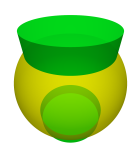
\includegraphics[width=0.6\linewidth]{union} \\ а)
  \end{minipage}
  \hfill
  \begin{minipage}[ht]{0.3\linewidth}\centering
    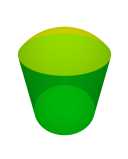
\includegraphics[width=0.6\linewidth]{intersection} \\ б)
  \end{minipage}
  \hfill
  \begin{minipage}[ht]{0.3\linewidth}\centering
    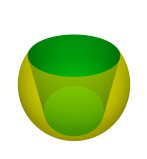
\includegraphics[width=0.6\linewidth]{difference} \\ в)
  \end{minipage}
  \caption{CSG операции}
  \label{fig:operations}  
\end{figure}

\section{CSG дерево} \label{sect_csg_tree}

CSG дерево это иерархическая модель в которой листовые узлы соответствуют базовым примитивам, а внутренние узлы "--- булевым операциям. Дочерним узлом внутреннего узла может быть примитив либо операция. Примитивы, в свою очередь, не имеют дочерних узлов. Корень дерева (узел не имеющий родительских узлов) соответствует объекту, который моделируется CSG деревом. Рисунок~\ref{fig:example_tree} изображает CSG модель, состоящую из сферы, параллелепипеда и двух цилиндров: $(((a \cap b) \setminus c) \setminus d)$. В этом примере узлы $a$, $b$, $c$ и $d$ являются примитивами (листовыми узлами), а остальные внутренними узлами.

Иерархические геометрические модели и CSG дерево, в частности, как правило, позволяют задать матрицу трансформации для любого из узлов. Таким образом, возможно задавать перенос, поворот и масштаб для отдельных примитивов и целых поддеревьев. По соглашению, трансформация применяется отностительно родительского узла и задает локальную систему координат для каждого узла дерева. Наличие локальной системы координат часто требуется для удобства интерактивного редактирования дерева и анимации.

CSG деревья обычно представляют как двоичные деревья "--- каждая операция имеет ровно два дочерних узла. Для сокращения записи можно использовать узлы произвольной арности ($\ge 2$), однако такое дерево всегда можно свести к бинарному.

\begin{figure} 
  \centering
  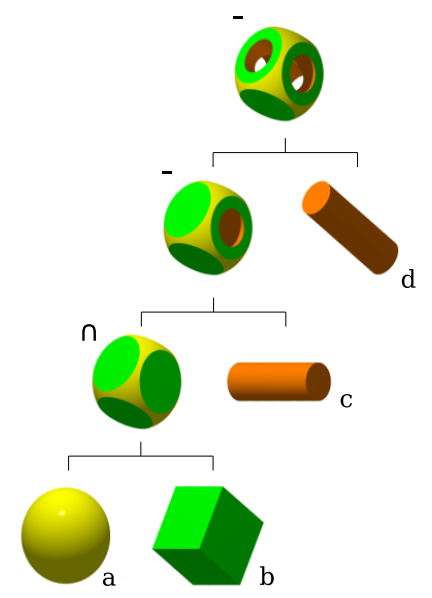
\includegraphics [scale=0.5] {example_tree}
  \caption{Пример CSG дерева}
  \label{fig:example_tree}
\end{figure}

\section{Обход} \label{sect_csg_traversal}

Алгоритмы на CSG деревьях, как правило, основаны на процедуре \textit{обхода} (англ. traversal) дерева "--- посещения каждого внутреннего и листового узла дерева в точности один раз. Обход начинается с корня дерева и доходит до листовых узлов рекурсивно. Такие обходы классифицируются по порядку, в котором узлы посещаются:

\begin{itemize}
  \item \textit{Прямой обход} (англ. pre-order traversal) посещает узел перед рекурсивным обходом левого и затем правого поддеревьев.

  \item \textit{Центрированный обход} (англ. in-order traversal) рекурсивно обходит левое поддерево, посещает текущий узел и далее правое поддерево.

  \item \textit{Обратный обход} (англ. post-order traversal) рекурсивно обходит левое и правое поддерево и затем посещает узел.
\end{itemize}

Центрированный обход можно использовать для получения CSG выражения для заданного дерева, слева направо. Например для CSG дерева на Рисунке~\ref{fig:example_tree} выражение будет выглядеть так: $(((a \cap b) \setminus c) \setminus d)$.

\section{Алгоритмы} \label{sect_csg_algo}

Настоящая работа сфокусирована на проблеме интерактивной визуализации конструктивных моделей, однако CSG подход позволяет эффективно решать ряд других задач геометрического моделирования. В данном разделе приводятся некоторые общие алгоритмы на CSG деревьях.

Задача \textit{классификации точки} (англ. point classification) состоит в том, чтобы определить в какой области пространства лежит заданная точка, внутри или снаружи CSG модели. Начиная с корня, рекурсивный обратный обход сначала классифицирует точку относительно дочерних узлов. Результат в каждом внутреннем узле определяется путем применения булевых операций к дочерним классификациям. Таким образом, классификация точки может быть реализована для сложных объектов, основываясь лишь на простых операциях классификации точки относительно примитивов.

Задача \textit{классификации линии} (англ. line classification) состоит в том, чтобы разделить линию на сегменты находящиеся внутри и снаружи CSG модели, а также точки находящиеся на поверхности модели. Классификация линии может быть выполнена схожим образом с классификацией точки, путем классификации линии относительно примитивов и применению булевой логики к дочерним интервалам на линии.

Задача \textit{бросания луча} (англ. ray casting) определяет первую точку пересечения заданного луча с поверхностью конструктивной модели. Эту задачу можно решить путем классификации линии и поиска ближайшей поверхности к началу луча в направлении луча. Однако, задача бросания луча является более частной чем задача классификация линии и может быть выполнена эффективнее. Эффективная реализация алгоритма бросания луча для CSG модели описана в Главе \ref{chapt3} и лежит в основе решения, описанного в настоящей работе.

Задача \textit{определения видимости} (англ. visibility query) может быть реализована с помощью бросания лучей.

Задача \textit{обнаружения столкновений} (англ. collision detection) требует определения области контакта, либо пересечения нескольких объектов. Пересечение CSG моделей может быть выражено как операция пересечения примененная к паре CSG моделей. Дальнейший анализ необходим для определения существования, а также конкретного вида области пересечения.

Задача \textit{выделения границы} (англ. boundary evaluation) сводится к переводу модели в граничное представление. В таком представлении поверхность модели задана явно в виде вершин, ребер и граней. Такое представление используется для расчета площади поверхности и прочих задач анализа поверхности, произведения геометрических операций, а также визуализации. Применимость операции выделения границы для задач интерактивной визуализации ограничивает трудоемкость этой операции для сложных моделей.

CSG модель также может быть представлена в воксельном представлении с заданной точностью. В этом представлении такие задачи как вычисление объема тела, классификация точки и бросания луча выполняются эффективнее. Однако, как и в случае с выделением границы, переход к воксельному представлению это ресурсоемкий процесс.

\section{Трансформация CSG дерева} \label{sect_csg_transform}

Узлы CSG дерева могут быть перемещены при сохранении того же объема и поверхности результирующей модели. Трансформация CSG дерева часто является необходимым предварительным шагом для последующей обработки и визуализации.

\subsection{Нормальная форма} \label{sect_csg_normalization}

Под нормализацией CSG дерева понимают приведение соответствующего CSG выражения к дизъюнктивной нормальной форме (дизъюнкция с минимальным числом элементарных конъюнкций). Эта процедура была предложена в работах \todo{Goldfeather et al. Stewart[36, 37]}. Переход к дизъюнктивной нормальной форме позволяет представить дерево в виде списка и обходить его без рекурсии (или стека). Такой подход позволяет использовать более простые алгоритмы визуализации, однако может приводить к экспоненциальному росту CSG дерева, значительно ограничивая  масштабируемость алгоритмов. Переход к CSG дереву в нормальной форме используется в таких алгоритмах визуализации CSG моделей как Trickle, Goldfeather и Sequenced Convex Subtraction.

\subsection{Позитивная форма} \label{sect_csg_positive_form}

Булево выражение представлено в \textit{позитивной форме}, если оно состоит только из операций дизъюнкции, конъюнкции и отрицания \todo{ours[9]}. Преобразование CSG дерева, соответствующего булеву выражению в позитивную форму может быть проведено с помощью законов де Моргана, которые в нотации теории множеств выглядят как:

\begin{align}
  \overline{x \cup y} & = \overline{x} \cap \overline{y}, \nonumber \\
  \overline{x \cap y} & = \overline{x} \cup \overline{y} \nonumber
\end{align}

Преобразования \ref{eq:positive}, основанные на законах де Моргана могут быть использованы для перехода к позитивной форме.

\begin{equation}
  \label{eq:positive}
  \begin{alignedat}{2}
    x \setminus y \  & \rightarrow \  x \cap \overline{y}, \\
    \overline{x \cup y} \  & \rightarrow \  \overline{x} \cap \overline{y}, \\
    \overline{x\cap y} \  & \rightarrow \  \overline{x} \cup \overline{y}, \\
    \overline{\overline{x}} \  & \rightarrow \  x
  \end{alignedat}
\end{equation}

Для перехода к позитивной форме используется прямой обход "--- преобразования применяются к текущему узлу, затем рекурсивно обходятся левое и правое поддеревья. В результате отрицания применяются к листовым узлам, а операции разности исчезают из дерева. Обратное преобразование к общей форме производится при обходе в обратном порядке (в этом случае отрицания исчезают из дерева).

В позитивной форме узлы CSG дерева могут быть перемещены на каждой операции объединения либо пересечения, благодаря коммутативности этих операций: $(a \cup b) = (b \cup a)$ и $(a \cap b) = (b \cap a)$. В то же время $(a \setminus b) = (b \setminus a)$, так как операция разности не коммутативна.

CSG деревья в позитивной форме используются во множестве CSG алгоритмов \todo{Stew[80, 77, 23, 78, 43, 46, 76]} включая алгоритмы визуализации. Среди преимуществ позитивной формы по сравнению с нормальной формой можно выделить структурную схожесть с исходным CSG деревом (количество узлов и их порядок в дереве не меняется) и отсутствие экспоненциального роста CSG дерева. Переход к позитивной формой необходим как предварительный шаг для таких методов визуализации CSG деревьев как BList \todo{Stew[78]} и CST \todo{Stew[46]}, а так же для метода описанного в настоящей работе.

\section{Алгебраическое упрощение CSG дерева} \label{sect_csg_tree_pruning}

CSG деревья часто могут быть упрощены путем отсечения поддеревьев, которые не вносят вклад в геометрическую форму объекта.

Булева алгебра может быть использована для упрощения CSG деревьев независимо от геометрических свойств модели. Преобразования \ref{eq:pruning} соответствуют возможным формам внутренних узлов, где $x$ представляет собой любой примитив или поддерево. При обратном обходе дерева, узлы соответствующие левой части преобразования заменяются на его правую часть.

\begin{equation}
  \label{eq:pruning}
  \begin{alignedat}{2}
    &x \cap x \  & \rightarrow \  &x, \\
    &x \cap \overline{x} \  & \rightarrow \  &\emptyset, \\
    &x \setminus x \  & \rightarrow \  &\emptyset, \\
    &x \cup x \  & \rightarrow \  &x, \\
    &x \cap \emptyset \  & \rightarrow \  &\emptyset, \\
    &x \setminus \emptyset \  & \rightarrow \  &x, \\
    &x \cap x \  & \rightarrow \  &x, \\
    &x \cup \emptyset \  & \rightarrow \  &x
  \end{alignedat}
\end{equation}

\section{Геометрическое упрощение CSG дерева} \label{sect_csg_bound_pruning}

\textit{Ограничивающие объемы} (англ. bounding volumes) и \textit{иерархии ограничивающих объемов} (англ. bounding volume hierarchies) являются важными инструментами для таких задач как визуализация \todo{Stew[24, 81, 96]} и обнаружение столкновений. Ограничивающие объемы также могут быть применены к задаче упрощения CSG дерева.

Ограничивающий объем полностью перекрывает геометрический объект вместе с дополнительным пространством. Такие задачи как классификация точки или бросание луча могут быть реализованы более эффективно для геометрически простых ограничивающих объемов, чем для более сложной геометрии, которую они содержат. Среди распространенных типов ограничивающих объемов можно выделить AABB (англ. Axis Aligned Bounding Box, ограничивающий параллелепипед параллельный осям), OBB (англ. Oriented Bounding Boxes, ориентированный ограничивающий параллелепипед), сферы и выпуклые оболочки. На практике, точность представления геометрии, производительность операций и сложность реализации различается для разных подходов к построению ограничивающих объемов. В то время как операции классификации точки и бросания луча могут быть выполнены очень быстро для AABB, они могут охватывать много лишнего пространства для геометрии ориентированной не параллельно координатным осям. Выпуклые оболочки, в свою очередь, гораздо лучше охватывают исходную геометрию, но их построение и алгоритмы классификации являются более вычислительно сложными. На практике, для задачи упрощения CSG дерева обычно используют AABB \todo{Stew[20, 37, 97]}, однако рассмотренные далее принципы применимы к любым видам ограничивающих объемов.

Для упрощения CSG дерева ограничивающие объемы определяются для каждого листового и внутреннего узла в обратном порядке обхода. Ограничивающие объемы листовых узлов вычисляются непосредственно по геометрии примитивов. Ограничивающие объемы внутренних узлов вычисляются по правилам \ref{eq:bounds}. Геометрическое упрощение дерева с использованием ограничивающих объемов следует проводить в общей форме CSG дерева, а не в позитивной, так как примитивы с отрицаниями не могут быть ограничены ограничивающим объемом конечного размера. 

\begin{equation}
  \label{eq:bounds}
  \begin{alignedat}{2}
    Bound(x \cap y) & = Bound(Bound(x) \cap Bound(y)), \\
    Bound(x \setminus y) & = Bound(Bound(x) \setminus Bound(y)), \\
    Bound(x \cup y) & = Bound(Bound(x) \cup Bound(y))
  \end{alignedat}
\end{equation}

Сам процесс упрощения CSG дерева также происходит во время обхода в обратном порядке. Узлы с пустыми ограничивающими объемами отбрасываются. Узлы с операциями пересечения и разности отбрасываются если пересечение ограничивающих объемов операндов соответствуют пустому объему.

Процесс вычисления ограничивающих объемов для внутренних узлов (согласно правилам \ref{eq:bounds}) может приводить к захватыванию ограничивающими объемами дополнительного пустого пространства, что нежелательно, так как в таком случае, поддеревья которые могли бы быть отброшены не будут отброшены. Однако, на практике, не смотря на ограничения, упрощение CSG дерева по ограничивающим объемам успешно используется (например, в работах \todo{Stew[20, 37, 97]}, а так же в настоящей работе).

\section{Определение пустого объекта} \label{sect_csg_null_object}

Задачи \textit{определения пустого объекта} (англ. Null Object Detection, NOD) и определения идентичного объекта (англ. Same Object Detection, SOD) возникают в областях геометрического моделирования, САПР, робототехники, компьютерной графики и компьютерного зрения. В контексте CSG NOD определяет, соответствует ли CSG дерево пустому объему. SOD определяет соответствуют ли два CSG дерева одному и тому же объему. Задачи SOD и NOD считаются эквивалентными, так как SOD может быть решена в терминах NOD: $SOD(a, b) = NOD(a \setminus b) \ \text{and} \ NOD(b \setminus a)$.

Подход к реализации NOD для CSG приведен в работе \todo{Tilove Stew[94]}.

Упрощение CSG дерева с помощью процедуры NOD вместо использования ограничивающих объемов, потенциально позволяет отсекать больше поддеревьев, так как NOD работает непосредственно с геометрией, а не с аппроксимациями. Следует отметить, что подобный подход требует гораздо больших вычислительных ресурсов, так как требует, в общем случае, перевода отдельных поддеревьев в граничное либо воксельное представление с заданной точностью.

\section{Алгоритм Кенслера} \label{sect2_kensler}

Подход к визуализации CSG моделей на базе трассировки лучей представленный в работе \todo{[8]} основан на поиске ближайших точек соударения лучей с примитивами 3D сцены. Алгоритм использует концепцию конечного автомата для вычисления точки пересечения с границей CSG модели. При этом требуется, чтобы базовые примитивы были замкнутыми (допустимо обобщение для ориентируемых поверхностей), имели согласованное поле нормалей и не содержали самопересечений. Элегантность решения и приемлемые ограничения позволяют довольно просто реализовать поддержку конструктивных моделей в любой программной системе, основанной на трассировке лучей. Хотя указанная работа не содержит упоминаний о практических испытаниях алгоритма, он представляется наилучшей основой для разработки специализированной версии для GPU. Далее кратко рассматриваются основные шаги алгоритма, в котором нами исправлены неточности в таблицах смены состояний.

Обозначим символом $T$ входное CSG дерево, а символами $L(T)$ и $R(T)$ его левое и правое поддерево соответственно. Для поиска ближайшей точки пересечения луча с деревом $T$, луч пересекается сначала с поддеревьями $L(T)$ и $R(T)$. Результатом каждого теста пересечения является одно из трех состояний луча: “вход” (entering), “выход” (exiting), “проходит мимо” (missing). На основе результатов двух  тестов, выполняется одно из трех действий: (1) вернуть точку соударения; (2) вернуть результат, соответствующий отсутствию пересечения; (3) переместить начальную точку луча к поддереву $L(T)$ или $R(T)$ и перейти на следующую итерацию для обработки очередной точки пересечения. В последнем случае, конечный автомат начинает новый цикл работы.

\begin{table} [ht]
    \caption{Таблицы перехода для булевых операций}
    \label{tbl:jump_table}
    \begin{SingleSpace}
    \setlength\extrarowheight{5pt} %вот этим управляем расстоянием между рядами, \arraystretch даёт неудачный результат
    \setlength{\tymin}{1.9cm}% минимальная ширина столбца
    \begin{tabulary}{\textwidth}{@{}>{\zz}L >{\zz}C >{\zz}C >{\zz}C@{}}% Вертикальные полосы не используются принципиально, как и лишние горизонтальные (допускается по ГОСТ 2.105 пункт 4.4.5) % @{} позволяет прижиматься к краям
        \toprule
        $\cup$       & Enter~$R(T)$                  & Exit~$R(T)$            & Miss~$R(T)$ \\
        \midrule
        Enter~$L(T)$ & RetLIfCloser \linebreak RetRIfCloser     & RetRIfCloser \linebreak LoopL & RetL \\
        Exit~$L(T)$  & RetLIfCloser \linebreak LoopR & LoopLIfCloser \linebreak LoopRIfCloser   & RetL \\
        Miss~$L(T)$  & RetR                          & RetR                          & Miss \\

        \toprule
        $\cap$       & Enter~$R(T)$                  & Exit~$R(T)$            & Miss~$R(T)$ \\
        \midrule
        Enter~$L(T)$ & LoopLIfCloser \linebreak LoopRIfCloser   & RetLIfCloser \linebreak LoopR & Miss \\
        Exit~$L(T)$  & RetRIfCloser \linebreak LoopL & RetLIfCloser \linebreak RetRIfCloser     & Miss \\
        Miss~$L(T)$  & Miss                          & Miss                          & Miss \\

        \toprule
        $\setminus$  & Enter~$R(T)$                  & Exit~$R(T)$            & Miss~$R(T)$ \\
        \midrule
        Enter~$L(T)$ & RetLIfCloser \linebreak LoopR & LoopLIfCloser LoopRIfCloser   & RetL \\
        Exit~$L(T)$  & RetLIfCloser \linebreak RetRIfCloser \linebreak FlipNormR & RetRIfCloser \linebreak FlipNormR \linebreak LoopL & RetL \\
        Miss~$L(T)$  & Miss                          & Miss                          & Miss \\
        \bottomrule
    \end{tabulary}%
    \end{SingleSpace}
\end{table}

В своей работе Кенслер предложил 3 таблицы переходов (по одной для каждой операции), которые контролируют смену состояний в процессе трассировки луча. В таблице 1 указаны откорректированные правила перехода, которые обеспечивают правильный результат визуализации во всех случаях. Псевдокод алгоритма Кенслера представлен на Рисунке \ref{fig:kensler}.

\begin{figure}[ht] 
  \centering
  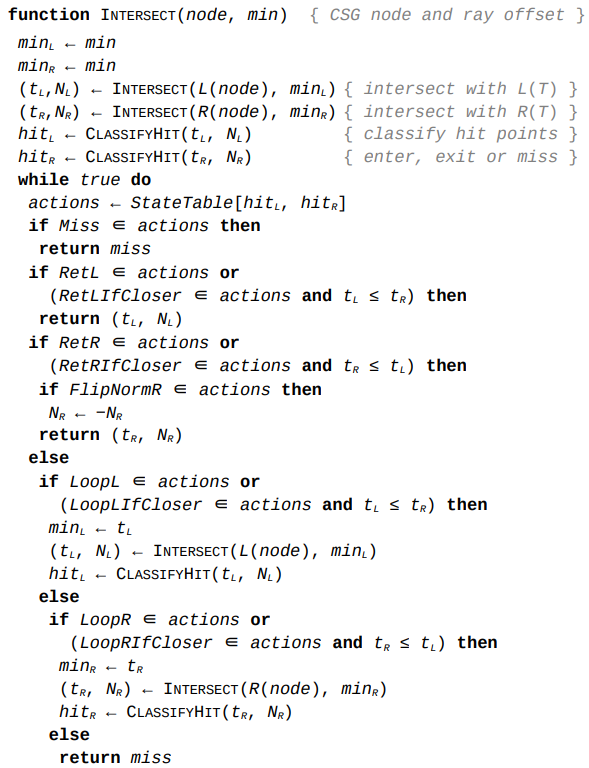
\includegraphics [scale=0.8] {algo_kensler}
  \caption{Рекурсивный алгоритм пересечения луча}
  \label{fig:kensler}
\end{figure}

Нетрудно видеть, что в таком виде алгоритм крайне плохо адаптирован для GPU, поскольку использует рекурсию и требует слишком много данных для сохранения состояния в стек. Однако его конвертация в итеративную форму, использующую стек минимального размера, является нетривиальной задачей и требует идентификации общих шаблонов и взаимосвязей во множестве путей исполнения алгоритма.

\section{Адаптация алгоритма для GPU} \label{sect2_kensler_gpu}

Основным результатом настоящего исследования является итеративный алгоритм пересечения луча с конструктивной геометрией, требующий минимального объема памяти для поддержания состояния и адаптированный для массивно-параллельных архитектур (включая графические). Основу данного алгоритма составляет высокоуровневый конечный автомат с магазинной памятью (англ. pushdown automaton, PDA), отвечающий за управление исходным алгоритмом Кенслера (рис. \ref{fig:highlevel_pda}).

\begin{figure}[ht] 
  \centering
  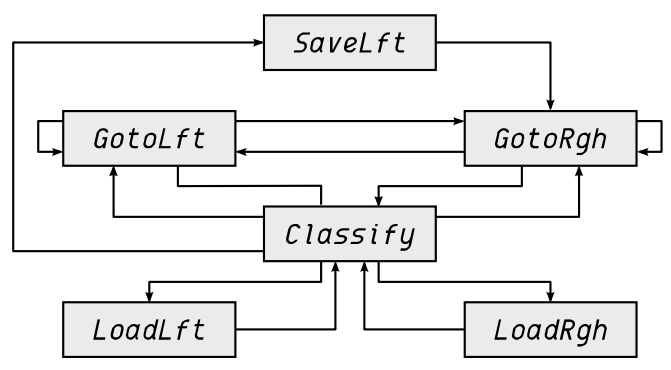
\includegraphics [scale=0.7] {highlevel_pda}
  \caption{Высокоуровневый конечный автомат}
  \label{fig:highlevel_pda}
\end{figure}

Применение таблиц смены состояний (табл. \ref{tbl:jump_table}) основано на результатах классификации точек пересечения с левым и правым поддеревом текущего узла CSG дерева. Поэтому все состояния высокоуровневого автомата можно разбить на два типа: (a) поиск точек пересечения с дочерними под-деревьями и (b) применение таблиц смены состояний для классификации полученных точек. К состояниям первого типа относятся: \textit{GotoLft} (поиск точки пересечения с левым поддеревом), \textit{GotoRgh} (поиск точки пересечения с правым поддеревом) и \textit{SaveLft} (сохранение атрибутов найденной точки пересечения с левым поддеревом в стек и переход к состоянию \textit{GotoRgh}). Последнее состояние необходимо по той причине, что поиск пересечения с правым поддеревом  приведет к перезаписи всех переменных функции, поэтому необходимые атрибуты пересечения быть сохранены для дальнейшего использования. Ко второму типу состояний относятся следующие: \textit{Classify} (применение таблиц смены состояний), \textit{LoadLft} (загрузка атрибутов точки пересечения с левым поддеревом из стека и переход к \textit{Classify}), \textit{LoadRgh} (загрузка атрибутов точки пересечения с правым поддеревом из стека и переход к \textit{Classify}). На псевдокоде алгоритм смены указанных состояний может быть записан как показано на Рисунке \ref{fig:iterative_intersect}.

\begin{figure}[ht] 
  \centering
  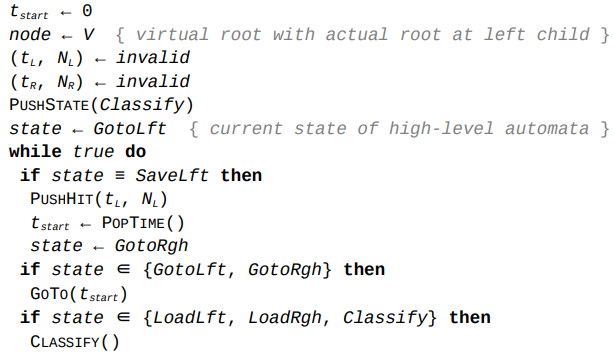
\includegraphics [scale=0.8] {iterative_intersect}
  \caption{Итеративная процедура пересечения}
  \label{fig:iterative_intersect}
\end{figure}

Вместо непосредственной обработки и хранения нормалей к примитивам в точках соударения, в данной реализации предлагается хранить \textit{знаковые} индексы соответствующих CSG примитивов (переменные $N_L$ и $N_R$). Такая модификация значительно уменьшает размер стека и позволяет получить больше информации на выходе алгоритма (в частности, индексы примитивов позволяют ассоциировать материалы с найденными точками соударения).

Функция \textit{GOTO()} вычисляет точки пересечения с левым и правым поддеревом (рис. \ref{fig:goto_code})), а функция \textit{CLASSIFY()} служит для классификации найденных точек с целью определения ближайшей точки, лежащей на границе конструктивного объекта (рис. \ref{fig:classify_code})). Отметим, что функция \textit{GOTO()} использует ограничивающие параллелепипеды узлов CSG дерева для оптимизации поиска точек пересечения.

\begin{figure}[ht] 
  \centering
  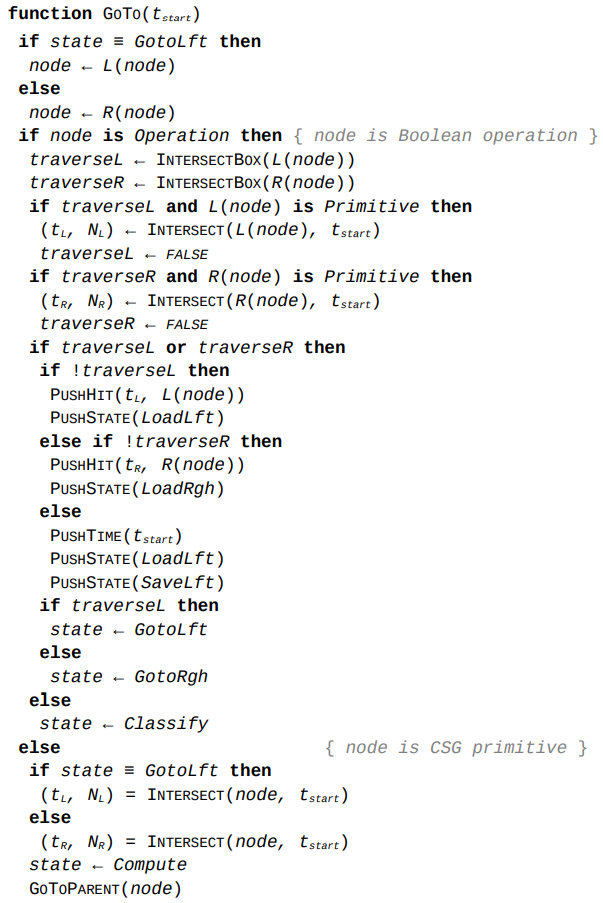
\includegraphics [scale=0.8] {goto_code}
  \caption{Псевдокод функции \textit{GOTO()}}
  \label{fig:goto_code}
\end{figure}

\begin{figure}[ht] 
  \centering
  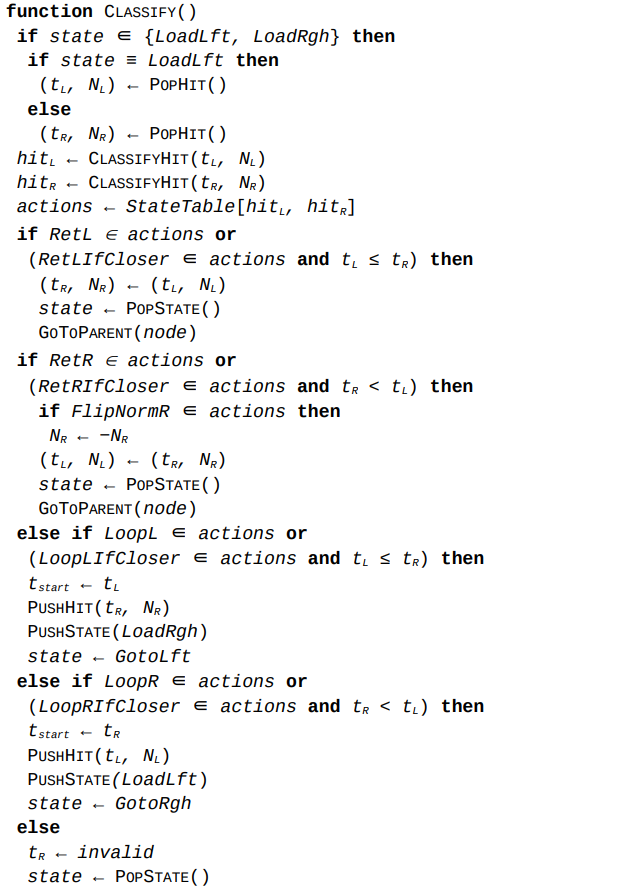
\includegraphics [scale=0.8] {classify_code}
  \caption{Псевдокод функции \textit{CLASSIFY()}}
  \label{fig:classify_code}
\end{figure}

В рамках настоящего исследования, данный алгоритм был реализован на базе фрагментных шейдеров OpenGL. При этом в практической реализации достаточно использовать  лишь два стека. Первый используется для хранения точек пересечения и индексов примитивов (функции \textit{PushTime} и \textit{PushHit}), в то время как второй используется для хранения состояний (функция \textit{PushState}).

\section{Оптимизация CSG дерева}

Очевидно, что производительность алгоритма сильно зависит от топологии CSG дерева, которая влияет непосредственно на высоту дерева, и на то как далеко в пространстве разнесены соседние элементы дерева (пространственная когерентность). Однако в конструктивной геометрии степень сбалансированности CSG дерева зависит прежде всего от действий пользователя. Таким образом, необходимо преобразовать исходное дерево $T$ в эквивалентное сбалансированное дерево $T'$  не увеличивая значительно число примитивов.
Предложена эффективная процедура оптимизации CSG деревьев, состоящая из 4 фаз: (1) преобразование исходного дерева в позитивную форму (см. раздел \ref{sect_csg_positive_form}); (2) пространственная оптимизация топологии дерева; (3) минимизация высоты дерева; (4) обратное преобразование дерева из позитивной формы.

\subsection{Пространственная сортировка CSG дерева} \label{sect2_spatial_sorting}

Для оптимальной производительности визуализации путём трассировки лучей необходимо использовать ограничивающие объёмы, как можно более плотно прилегающие к узлам CSG дерева. Такой выбор ограничивающих объёмов минимизирует вероятность их пересечения с лучом, не ведущего к последующему пересечению с узлом дерева. Предложена процедура пространственной оптимизации CSG дерева, минимизирующая размер ограничивающих объёмов внутренних узлов дерева. Назовём трилетом выбранный узел дерева вместе с набором его непосредственных узлов-потомков (поддерево ограниченное снизу). Предложенная процедура оптимизации основана на последовательном выборе трилетов, состоящих из узлов с одинаковыми булевыми операциями,  и их последующей реструктуризации (в позитивной форме узлы таких трилетов могут быть произвольно перемещены внутри трилета). Трилеты могут быть построены во время прямого обхода CSG дерева путём рекурсивного объединения узлов с одинаковыми CSG операциями. Полученный трилет необходимо реорганизовать с помощью эвристики площади поверхности (Surface Area Heuristic, SAH), широко используемой для построения ускоряющих структур таких как k-d дерево или иерархия ограничивающих объёмов (BVH). Затем процедура продолжается рекурсивно с листовыми узлами трилета.

Реорганизация трилета происходит с помощью техники корзин схожей с техникой построения BVH \todo{ours[10]}. Структура BVH строится по листовым узлам трилета, ограниченным AABB (ограничивающий параллелепипед параллельный осям) полученным из исходного CSG дерева в общей форме. Для листовых узлов трилета соответствующих примитивам CSG дерева с отрицаниями используются исходные ограничивающие объёмы, а не их дополнения, которые соответствовали бы бесконечному AABB. Такая стратегия позволяет немного улучшить результат, так как бесконечные ограничивающие объёмы не несут никакой информации о позиции примитивов.

\subsection{Минимизация высоты CSG дерева} \label{sect2_height_minimization}

Предложенный алгоритм вычисляет точку пересечения итеративно с использованием стека. Однако на устройствах  с массивно-параллельной архитектурой, таких как графические процессоры, поддержка отдельного стека для каждого из множества процессов ведёт к значительным затратам памяти и пропускной способности интерфейса памяти. Чтобы минимизировать размер стека, необходимо преобразовать исходное CSG дерево в эквивалентное сбалансированное дерево. В качестве очередной стадии оптимизации дерева, предложено уменьшить высоту CSG дерева с помощью локальных преобразований. На этом этапе оптимизации, рассматриваются два типа трилетов. Для краткости, назовём узел-потомок данного узла с наибольшей высотой (в исходном дереве $T$) тяжёлым потомком. Первый тип рассматриваемых трилетов предполагает одинаковую CSG операцию ($\cup$ или $\cap$) в корне трилета $N_1$ и его тяжёлом потомке $N_2$ (см. Рисунок \ref{fig:tree_rotations} (а)). Пусть $T_3$ является тяжёлым потомком $N_2$. Тогда, очевидно, если $h(T_3) > h(T_1) + 1$ предпочтительно поменять эти поддеревья местами. По аналогии с поворотами в двоичных деревьях поиска, такая операция ведёт к предсказуемому уменьшению высоты поддерева с корневым узлом $N_1$ на 1.

\begin{figure}[ht]
  \begin{minipage}[ht]{0.49\linewidth}\centering
    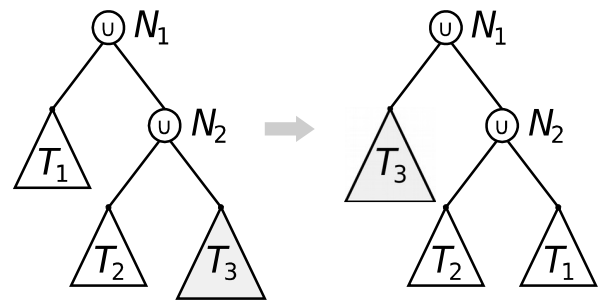
\includegraphics[width=0.8\linewidth]{tree_rot1} \\ а)
  \end{minipage}
  \hfill
  \begin{minipage}[ht]{0.49\linewidth}\centering
    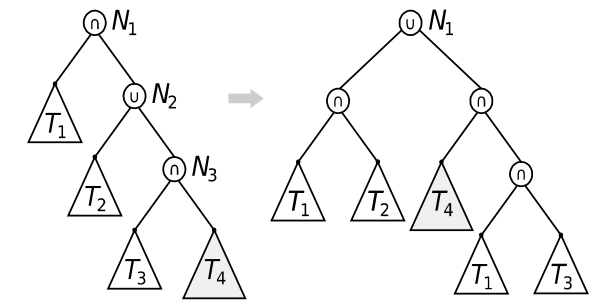
\includegraphics[width=0.8\linewidth]{tree_rot2} \\ б)
  \end{minipage}
  \caption{Оптимизация первого и второго типов}
  \label{fig:tree_rotations}  
\end{figure}

Второй тип трилетов, соответствует ситуации, когда операции в корневом узле $N_1$, его тяжёлом потомке $N_2$ и последующем тяжёлом потомке $N_3$ перемежаются (например $\cup-\cap-\cup$ или $\cap-\cup-\cap$). Рассмотрим последовательность $\cup-\cap-\cup$ (см. Рисунок \ref{fig:tree_rotations} (б)). В этом случае трилет с корнем $N_1$ может быть описан выражением: $T_1 \cap (T_2 \cup T_3 \cup T_4) = (T_1 \cap T_2) \cup (T_1 \cap T_3 \cap T_4)$. Пусть $T_4$ является тяжёлым потомком $N_3$. Тогда если $h(T_4) > h(T_1) + 2$, то указанное выше преобразование позволяет сократить высоту трилета на 1. Заметим, что указанное преобразование локально и не влияет на другие узлы дерева. Однако, такая оптимизация нежелательна, так как она приводит к дублированию поддерева $T_1$. В предложенном решении такая оптимизация высоты дерева используется только когда невозможно больше применять оптимизации первого типа. Преобразования применяются к дереву итеративно, на каждой итерации подходящие преобразования применяются к поддеревьям во время обхода в обратном порядке.

\section{Реализация эффектов глобального освещения}

Современный подход к инженерной графике включает в себя расширение визуализации геометрии за счет эффектов глобального освещения. Тем самым повышается наглядность и удобство восприятия, особенно для сложных моделей.

Существующие подходы как правило ограничиваются частичной поддержкой эффектов глобального освещения для интерактивной визуализации. Используются такие подходы как SSAO и отражения с использованием карт окружения. Однако, для многих задач требуется полноценный расчет глобального освещения.

В настоящей работе используется трассировка лучей как основной метод визуализации CSG деревьев. Реализованная операция бросания луча позволяет естественным образом расширить подход для расчета глобального освещения используя (стохастическую) трассировку путей, которая решает уравнение визуализации методом Монте-Карло.

\subsection{Реализация трассировки лучей Уиттеда}

Классическая трассировка лучей (или трассировка лучей Уиттеда) остается одним из самых популярных методов визуализации. Данная техника поддерживает базовые эффекты глобального освещения и является частным случаем стохастической трассировки путей, она может применяться для быстрой технической визуализации в САПР.

\textit{Прямое освещение}. Расчет прямого освещения выполняется аналогично стохастической трассировке путей, что обеспечивает корректный расчет теней. Обычно допускаются только точечные и направленные источники света, что не позволяет реализовать эффект мягких теней в этом режиме, стохастические методы моделирования заменяются детерминированными.

\textit{Идеальные отражения и преломления}. Обычно данные типы отражения и преломления являются единственными вторичными эффектами, которые можно получить в классической трассировке лучей. Для моделирования данных эффектов применяются детерминированные методы. В настоящей работе трассировка лучей Уиттеда применяется как вспомогательный метод для быстрого отображения массивных CSG сцен.

\subsection{Двунаправленная трассировка путей}

В стохастической трассировке путей все траектории переноса излучения генерируются «прямым» методом, начиная от диафрагмы виртуальной камеры. Данная стратегия не всегда является наиболее эффективной. Характерными примерами служат сцены с преобладанием вторичного освещения (перекрытые источники света) или резкими колебаниями светового поля (каустики). В подобных случаях крайне сложно построить корректные пути переноса излучения, выполняя трассировку от виртуальной камеры.

Решить данную проблему можно за счет двунаправленной трассировки путей, которая была независимо предложена Э. Вичем \todo{D[129]} и Э. Лафорчуном \todo{D[6]}. Данный метод генерирует пути из источника света («световой» путь) и диафрагмы виртуальной камеры («видовой» путь). Затем все вершины построенных путей соединяются теневыми лучами, за счет чего образуется множество корректных путей переноса излучения.

В двунаправленной трассировке каждый путь длины $k$ можно построить $k + 1$ способом, соединяя «видовой» путь длины $s \ge 0$ со «световым» путем длины $t \ge 0$, где $k = s + t$. При этом любой из двух путей может быть нулевой длины. Если длина «светового» пути равна нулю, то последовательность «видовых» вершин является неявным путем и должна заканчиваться на источнике света. Если «видовой» путь имеет нулевую длину (содержит только одну вершину), то «световой» путь явно соединяется с виртуальной камерой. В настоящей работе не рассматривается ситуация, когда «световой» путь непосредственно пересекает диафрагму виртуальной камеры. Как правило, вклад таких путей в окончательное изображение пренебрежимо мал.

Стандартный вариант двунаправленной трассировки путей является достаточно ресурсоемкой техникой для реализации на графическом процессоре. Для вычисления вкладов отдельных комбинированных путей необходимо сохранить \textit{все} вершины «светового» и «видового» пути. Затраты памяти на один луч для двунаправленной трассировки более чем в 20 раз могут превосходить соответствующие затраты памяти для обычной трассировки путей. В результате для синтеза изображения размером 1024 x 1024 пикселей необходимо свыше 3 Гб памяти только для хранения двунаправленных семплов. Проблема может быть частично решена за счет обработки изображения порциями небольшого размера. Однако для эффективной балансировки нагрузки и утилизации ресурсов графический процессор должен обрабатывать потоки данных, число элементов которых как минимум в несколько раз выше по сравнению с максимальным числом одновременно работающих потоков (десятки тысяч). С учетом этого нижнего ограничения затраты памяти остаются весьма значительными и не опускаются ниже $\sim$ 500 Мб. Следует учитывать, что для обработки некоторых сцен (таких как крупный план прозрачного объекта) максимальной длины 16 может оказаться недостаточно, что приведет к смещенной оценке изображения (или к росту потребления памяти). С другой стороны, современные графические карты снабжаются относительно небольшим объемом памяти (1–4 Гб), которую необходимо максимально экономно использовать для хранения геометрии сцены, ускоряющей структуры и текстур.

\subsection{Алгоритм «усеченной» двунаправленной трассировки путей}

В силу перечисленных обстоятельств в настоящей работе предлагается использовать «усеченный» вариант двунаправленной трассировки путей, который по затратам сопоставим с обычной трассировкой и сохраняет основные преимущества исходного алгоритма. Данный алгоритм формирует изображение за два этапа. На первом этапе выполняется обратная трассировка от объектива виртуальной камеры, в ходе которой генерируются явные и неявные траектории переноса излучения. На втором этапе выполняется прямая трассировка от источника света, в процессе которой все вершины пути явно соединяются с камерой. Вклады различных путей комбинируются в одну несмещенную Монте-Карло оценку с использованием многократной выборки по значимости. Данный метод можно рассматривать как частный случай «полной» двунаправленной трассировки, при котором один из соединяемых путей содержит не более одной вершины ($s \le 1$ или $t \le 1$). Основные преимущества такого подхода определяются следующими особенностями:

\begin{itemize}  
  \item На стадии прямой и обратной трассировки для обработки путей произвольной длины требуется фиксированный объем памяти. Данное обстоятельство позволяет нагрузить графический процессор большим числом «легковесных» путей и снимает ограничения при синтезе несмещенных изображений (когда необходимо большое число отскоков).
  
  \item Трассировка путей в каждом направлении выполняется независимо, что обеспечивает широкие возможности распараллеливания. Например, «прямой» и «обратный» проход визуализации можно выполнять на различных графических процессорах без какого-либо взаимодействия в ходе вычислений (для получения результата два изображения достаточно просто сложить).
  
  \item Полностью исключается трудоемкая фаза соединения «прямого» и «обратного» путей (требует информации обо всех вершинах каждого пути).
  
  \item Значительно упрощается реализация многократной выборки по значимости, которая позволяет оптимально скомбинировать вклады прямых и обратных путей.
\end{itemize}
           % Глава 2
\chapter{Программный комплекс для интерактивной визуализации сложных сцен конструктивно-блочной геометрии на графических процессорах и его экспериментальное исследование} \label{chapt3}

Данная глава посвящена экспериментальному исследованию разработанного комплекса и отвечает следующим целям:
\begin{itemize}
  \item Представить описание состава и структуры разработанного программного комплекса для интерактивной визуализации сложных сцен конструктивно-блочной геометрии на графических процессорах, который реализует положения главы 2 с использованием инструментов программирования параллельных графических архитектур.

  \item Экспериментально проверить корректность моделирования глобального освещения в сцене путем сравнения результатов моделирования с эталонными изображениями.

  \item Дать оценку производительности программного комплекса, а также оценку эффективности предложенных решений относительно аналогов.
\end{itemize}

\section{Состав и структура программного комплекса для интерактивной визуализации сложных сцен конструктивно-блочной геометрии на графических процессорах}

\subsection{Высокопроизводительные свободно распространяемые библиотеки нижнего уровня}

В разработанном программном комплексе активно применяются следующие свободно распространяемые библиотеки:

\begin{itemize}
    \item Eigen [http://eigen.tuxfamily.org]. Библиотека шаблонов на языке C++ для линейной алгебры. Характеризуется универсальностью, высоким уровнем производительности, лаконичностью программных интерфейсов (вектора и матрицы) и поддержкой многих компиляторов. Высокое быстродействие достигается посредством применения SIMD-расширений ЦПУ и техник метапрограммирования (таких как Expression Templates). Библиотека доступна с исходным кодом по лицензиям LGPL3 и GPL2.
    \item Boost [http://www.boost.org]. Собрание библиотек, расширяющих язык C++ подобно STL (Standard Template Library). Библиотеки Boost ускоряют массу задач прикладного программирования, предоставляя типичные алгоритмы, контейнеры данных, «умные указатели», примитивы многопоточного программирования и многое другое. Данные библиотеки доступны с исходным кодом по лицензии Boost Software License.
    \item Qt [http://qt-project.org]. Кросс-платформенный инструментарий разработки ПО на языке C++. Содержит основные классы, которые могут потребоваться при разработке прикладного программного обеспечения, включая элементы графического интерфейса пользователя. Инструментарий Qt является полностью объектно-ориентированным и поддерживает технологию компонентного программирования. Библиотека доступна с исходным кодом по лицензиям GPL3 и LGPL.
    \item GLog [http://code.google.com/p/google-glog]. Вспомогательная библиотека на языках C/C++, которая позволяет записывать в журнал приложения указанные разработчиком события (application-level logging). Данный функционал позволяет упростить отладку и выявление проблем. Библиотека распространяется с исходным кодом по лицензии New BSD.
    \item GLEW [http://sourceforge.net/projects/glew]. Мультиплатформенная библиотека на языке C для работы с расширениями OpenGL (поддерживает версию 4.3). Доступна с исходным кодом по лицензиям BSD и MIT.
    \item GLFW [http://www.glfw.org/index.html]. Мультиплатформенная библиотека на языке C для создания контекста OpenGL и управления вводом, включая клавиатуру, мышь и джойстик. Распространяется с исходным кодом по лицензии zlib/libpng.
\end{itemize}

Наряду с указанными библиотеками в разработанном комплексе применяются инструменты программирования графических процессоров предоставляемые интерфейсом программирования OpenGL.

\subsection{Структура программного комплекса и состав его библиотек прикладных программ}

Разработанный программный комплекс состоит из набора модулей, которые основаны на перечисленных выше базовых библиотеках (рис. \ref{fig:arch}). На нижнем слое функциональности расположена библиотека Graphics. Библиотека Graphics отвечает за поддержку типовых задач программирования 3D графики OpenGL, включая управление виртуальными камерами и устройствами ввода, загрузку изображений, настройку шейдерных программ и буферов кадров. Основная функциональность программного комплекса содержится в библиотеках \textit{CSG} и \textit{Renderer}. Библиотека \textit{CSG} реализует рассмотренное в главе 2 иерархическое представление CSG сцены, а также описания материалов и источников света. Библиотека \textit{Renderer} реализует программный конвейер трассировки лучей (путей). Верхний слой функциональности представлен библиотеками \textit{Convert} и \textit{GUI}, которые отвечают за импорт моделей CSG сцен (во внутренний формат системы) и содержат некоторые элементы графического интерфейса Qt (многорежимное окно визуализации с возможностью переключения между различными режимами визуализации).

\begin{figure}[ht]
  \centering
  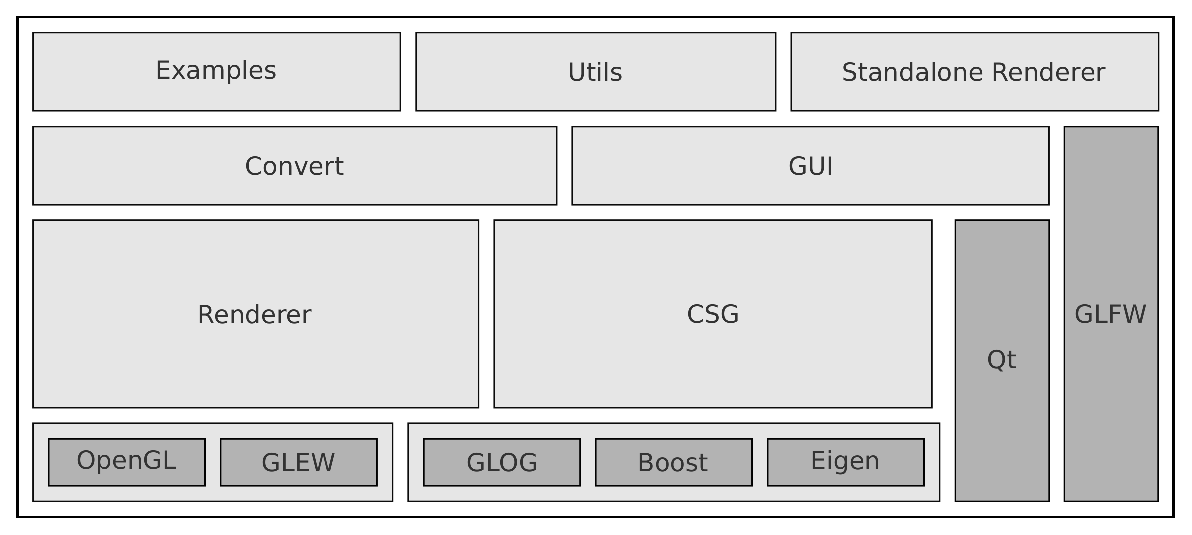
\includegraphics [scale=0.8] {arch}
  \caption{Основные компоненты разработанного программного комплекса}
  \label{fig:arch}
\end{figure}

На основе верхнего уровня функциональности разрабатываются различные клиентские программы, включая тестовые и демонстрационные приложения, а такде специализированные системы визуализации. На данный момент разработан автономный визуализатор с возможностью редактирования CSG сцены.

В совокупности разработанные библиотеки и приложения содержат свыше 50 файлов программного кода (более 10 000 строк).

\section{Исследование производительности программного комплекса} \label{sect_results}

Оценки производительности для данного исследования были получены на графических процессорах: NVIDIA GeForce GTX 680, AMD Radeon HD 7870 и Intel HD 4000. Измерения проводились при отрисовке в окно размером 1280 x 720. Первая сцена для тестирования предложенного алгоритма представляет собой CSG модель города (см. Рисунок \ref{fig:results_city}). Во всех вариантах сцена составлена как одно CSG дерево (схожие элементы добавлены с помощью операции объединения). В простейшей конфигурации (в) модель состоит из 3385 примитивов. Более сложные варианты сцены (г), (д) и (е) состоят из 86К, 343К и 987К примитивов соответственно. Рисунок (б) представляет собой пример сложного для альтернативных решений ракурса, с большим числом слоёв глубины. Сцена «Город», представленная в трёх вариантах позволяет проанализировать зависимость производительности предложенного алгоритма от сложности CSG модели. Для каждого графического процессора результаты представлены в виде двух столбцов (см. Таблицу \ref{tbl:timings}): левый соответствует измеренному значению величины отображённых кадров в секунду (Frames Per Second, FPS) без пространственной оптимизации дерева ($-$), правый содержит значения, полученные с выполненной пространственной оптимизацией ($+$).

\begin{figure}[ht]
  \begin{minipage}[ht]{0.49\linewidth}\centering
    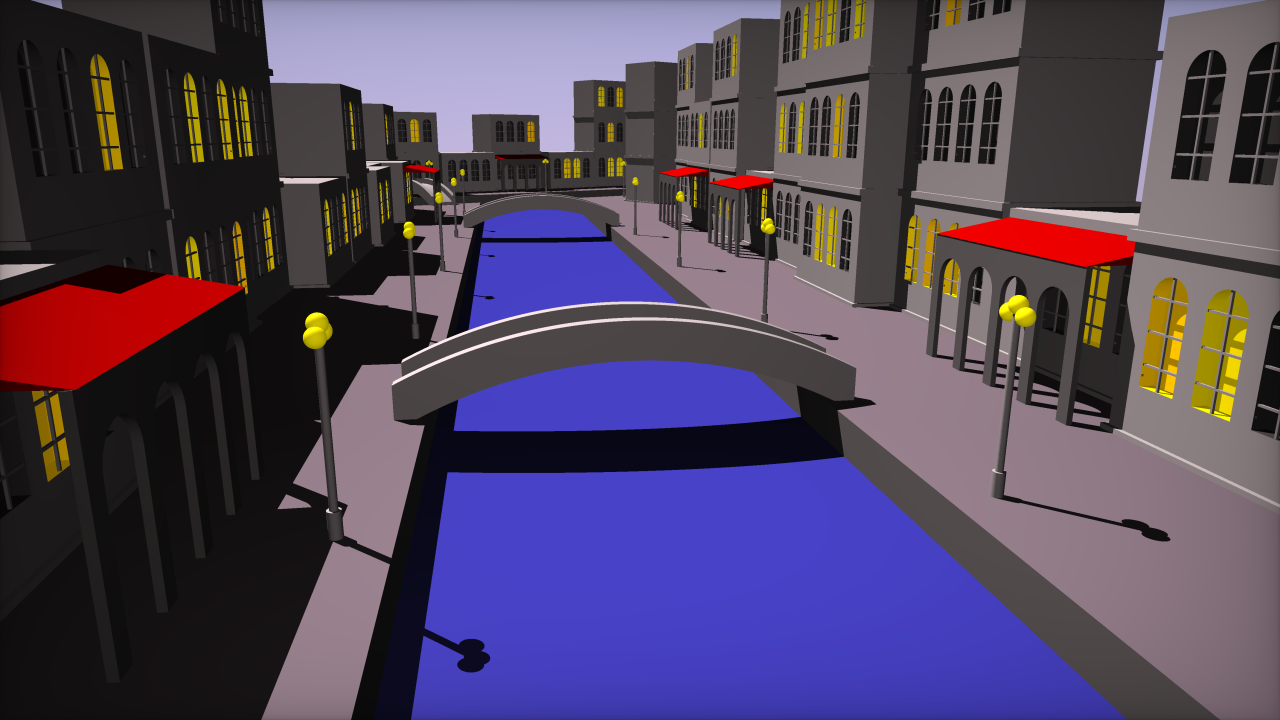
\includegraphics[width=0.95\linewidth]{screenshot_41} \\ а)
  \end{minipage}
  \hfill
  \begin{minipage}[ht]{0.49\linewidth}\centering
    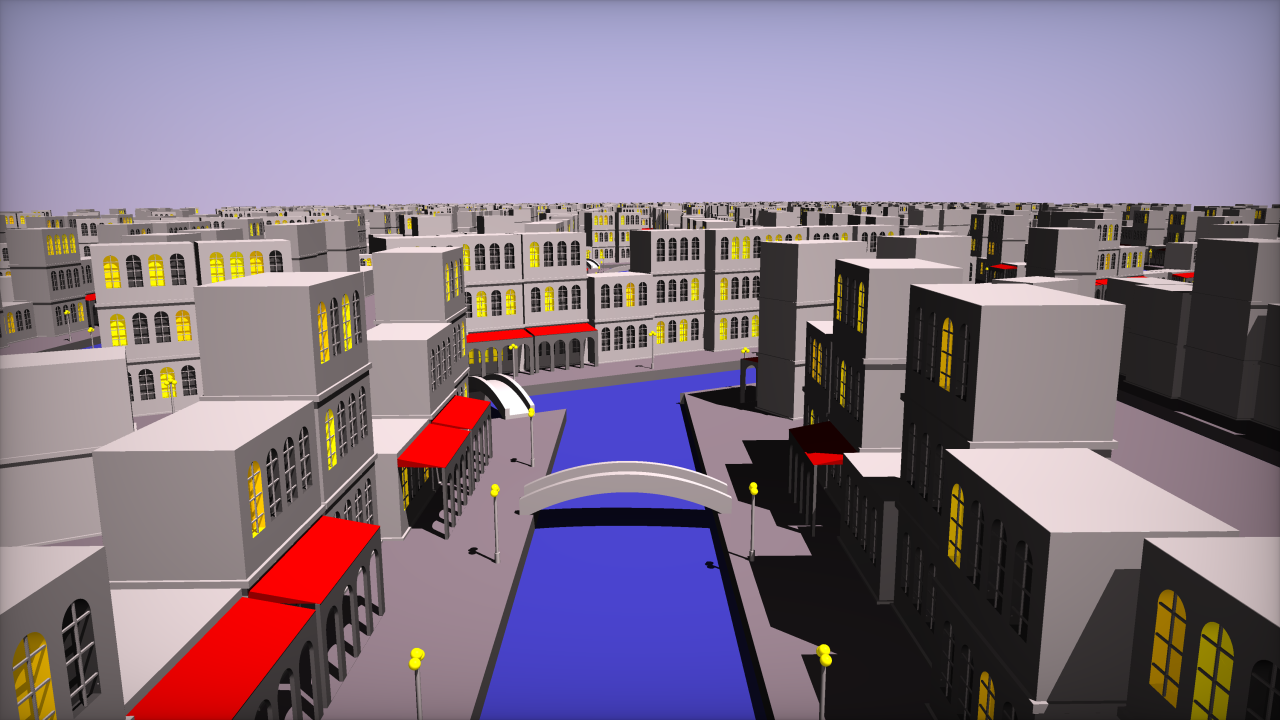
\includegraphics[width=0.95\linewidth]{screenshot_27} \\ б)
  \end{minipage}

  \begin{minipage}[ht]{0.49\linewidth}\centering
    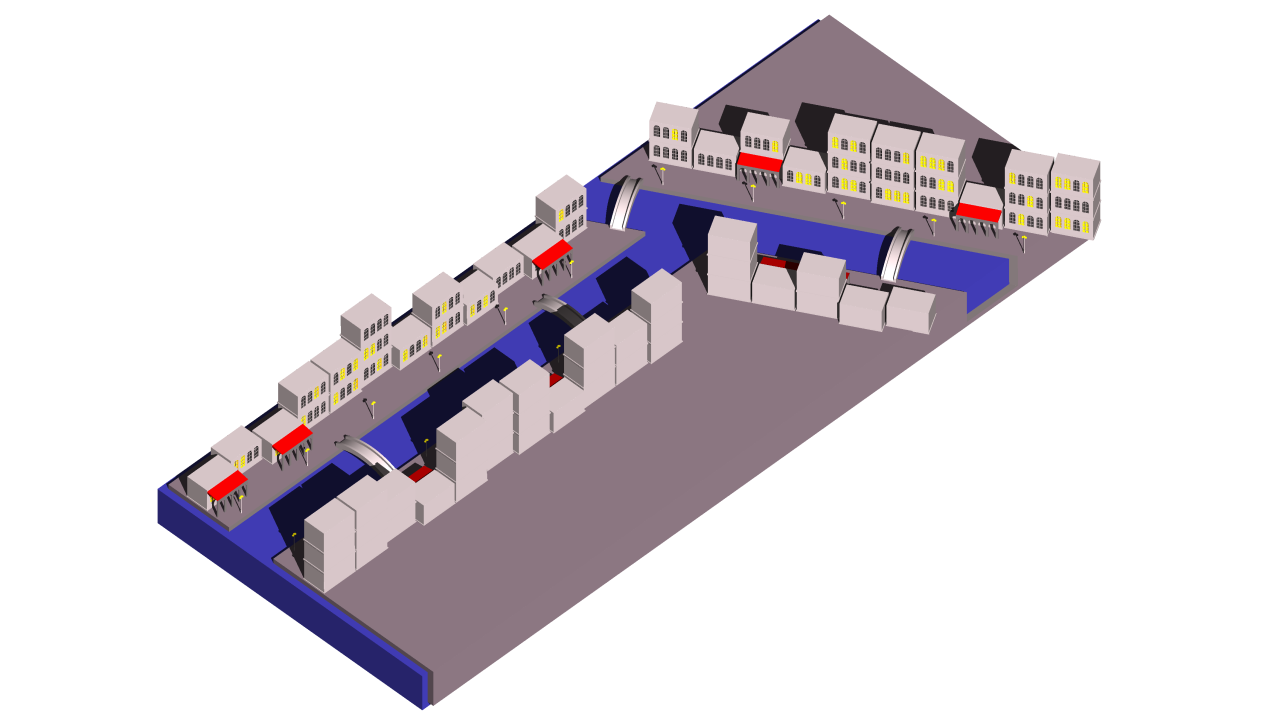
\includegraphics[width=0.95\linewidth]{screenshot_24} \\ в)
  \end{minipage}
  \hfill
  \begin{minipage}[ht]{0.49\linewidth}\centering
    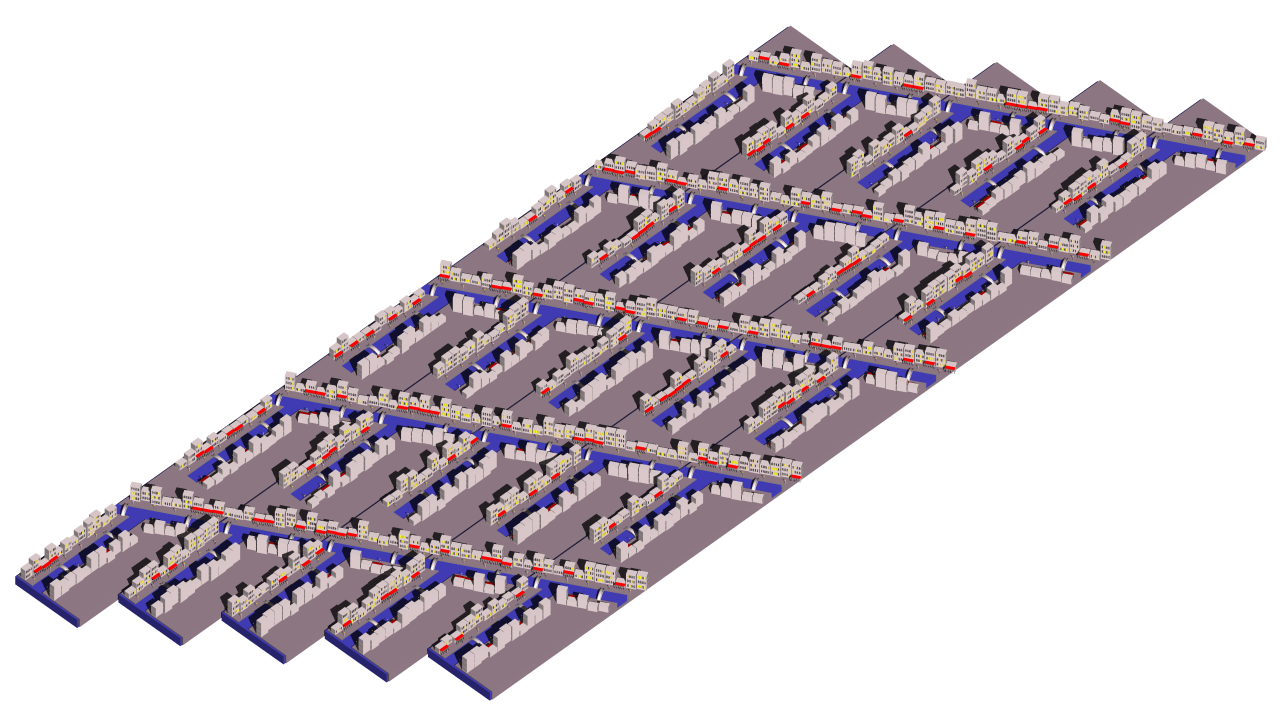
\includegraphics[width=0.95\linewidth]{screenshot_29} \\ г)
  \end{minipage}

  \begin{minipage}[ht]{0.49\linewidth}\centering
    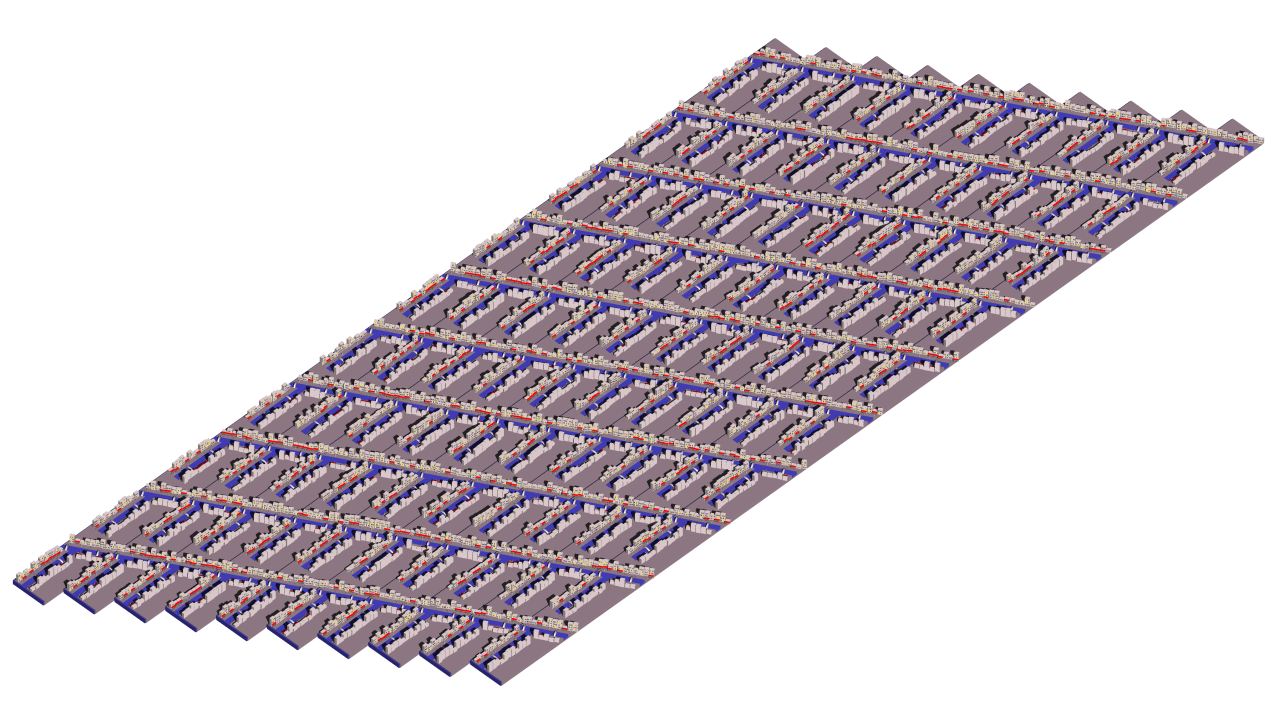
\includegraphics[width=0.95\linewidth]{screenshot_26} \\ д)
  \end{minipage}
  \hfill
  \begin{minipage}[ht]{0.49\linewidth}\centering
    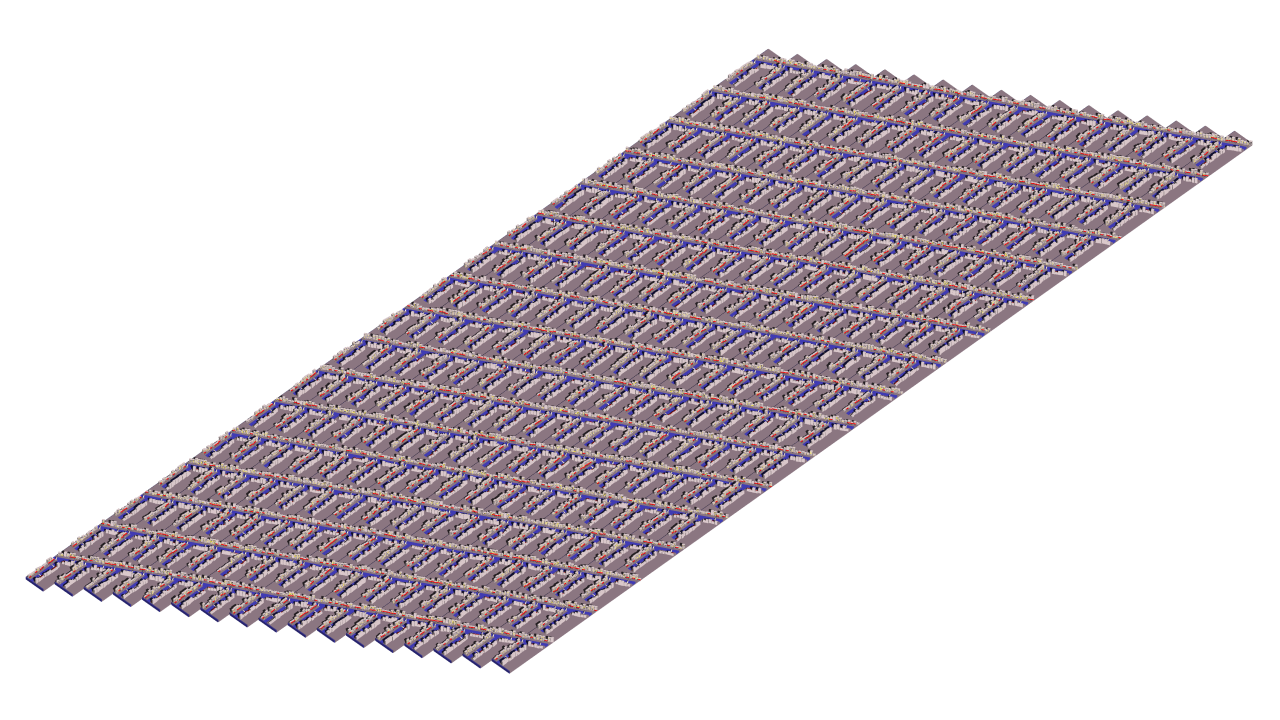
\includegraphics[width=0.95\linewidth]{screenshot_28} \\ е)
  \end{minipage}
  \caption{Сцена «Город»}
  \label{fig:results_city}  
\end{figure}

\begin{table} [ht]
    \caption{Оценки производительности}
    \label{tbl:timings}
    \begin{SingleSpace}
    \setlength\extrarowheight{5pt} %вот этим управляем расстоянием между рядами, \arraystretch даёт неудачный результат
    \setlength{\tymin}{1.9cm}% минимальная ширина столбца
    \begin{tabulary}{\textwidth}{@{}>{\zz}L >{\zz}C >{\zz}C >{\zz}C >{\zz}C >{\zz}C >{\zz}C >{\zz}C >{\zz}C@{}}
    	\toprule
		\multirow{3}{*}{Сцена} & \multirow{3}{*}{Примитивы} & \multirow{3}{*}{Глубина дерева} & \multicolumn{2}{c}{\textit{Int4000}} & \multicolumn{2}{c}{\textit{Rad7870}} & \multicolumn{2}{c}{\textit{GF680}}\\
		\cline{4-9}
		& & & $-$ & $+$ & $-$ & $+$ & $-$ & $+$\\
		\midrule
		Город (\textit{a}) & 3385   & 14 & 7   & 7.5 & 50  & 60 & 51  & 57\\
		Город (\textit{b}) & 343589 & 22 & 1.8 & 4.5 & 6.5 & 17 & 8   & 22 \\
		Город (\textit{c}) & 3385   & 14 & 21  & 22  & 66  & 68 & 120 & 125\\
		Город (\textit{d}) & 86673  & 20 & 8   & 11  & 21  & 25 & 31  & 38 \\
		Город (\textit{e}) & 343589 & 22 & 4.5 & 8   & 12  & 19 & 15  & 27 \\
		Город (\textit{f}) & 987218 & 24 & 2.3 & 7   & 6.7 & 18 & 8.3 & 21 \\

		\midrule

		Сыр (\textit{a}) & 1002  & 11 & 0.4        & 17  & 4.6        & 110  & 5.8        & 128\\
		Сыр (\textit{b}) & 8002  & 14 & \tiny{N/A} & 6.5 & 0.5        & 28   & 0.5        & 32 \\
		Сыр (\textit{c}) & 32002 & 17 & \tiny{N/A} & 0.5 & \tiny{N/A} & 3.7  & \tiny{N/A} & 4 \\

		\midrule

		Спутники (\textit{a}) & 87565   & 7 & 5    & 9    & 26  & 67  & 29  & 65 \\
		Спутники (\textit{b}) & 1120065 & 7 & 2.8  & 4.5  & 8   & 18  & 7  & 15 \\
		Спутники (\textit{c}) & 1120065 & 7 & 2.5  & 4.5  & 4.2 & 9   & 5.6 & 12 \\
		\bottomrule
    \end{tabulary}%
    \end{SingleSpace}
\end{table}

Вторая сцена для тестирования алгоритма представляет собой CSG модель «Швейцарского сыра» с дырами различного размера, смоделированными с помощью сфер (см. Рисунок~\ref{fig:results_cheese}). Число дыр возрастает с 1000 (а) до 8000 (б), и до 32000 (в) приводя к увеличению количества пересекающихся примитивов и сложности вычисления принадлежности точки определённой поверхности. В результате, производительность отрисовки модели «Швейцарский сыр» алгоритмом сильно зависит от успеха пространственной сортировки CSG дерева (см. Таблицу~\ref{tbl:timings}).

\begin{figure}[ht]
  \begin{minipage}[ht]{0.325\linewidth}\centering
    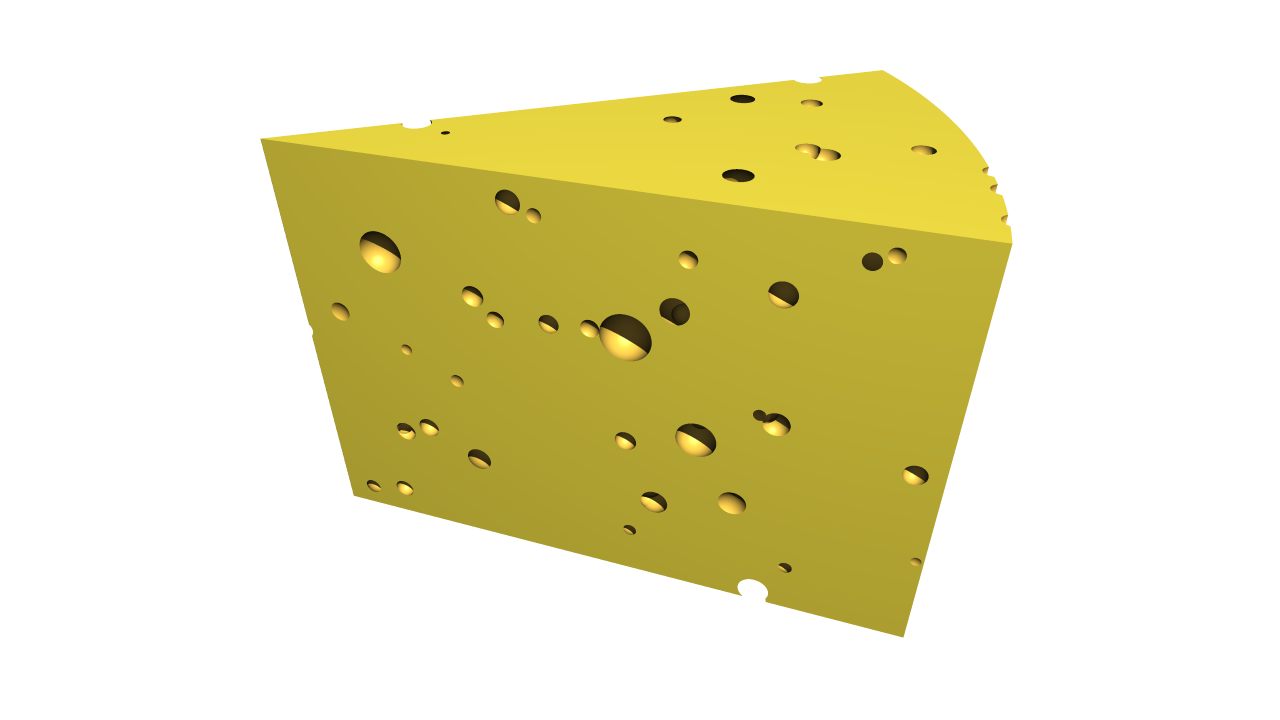
\includegraphics[width=0.95\linewidth]{screenshot_23} \\ а)
  \end{minipage}
  \hfill
  \begin{minipage}[ht]{0.325\linewidth}\centering
    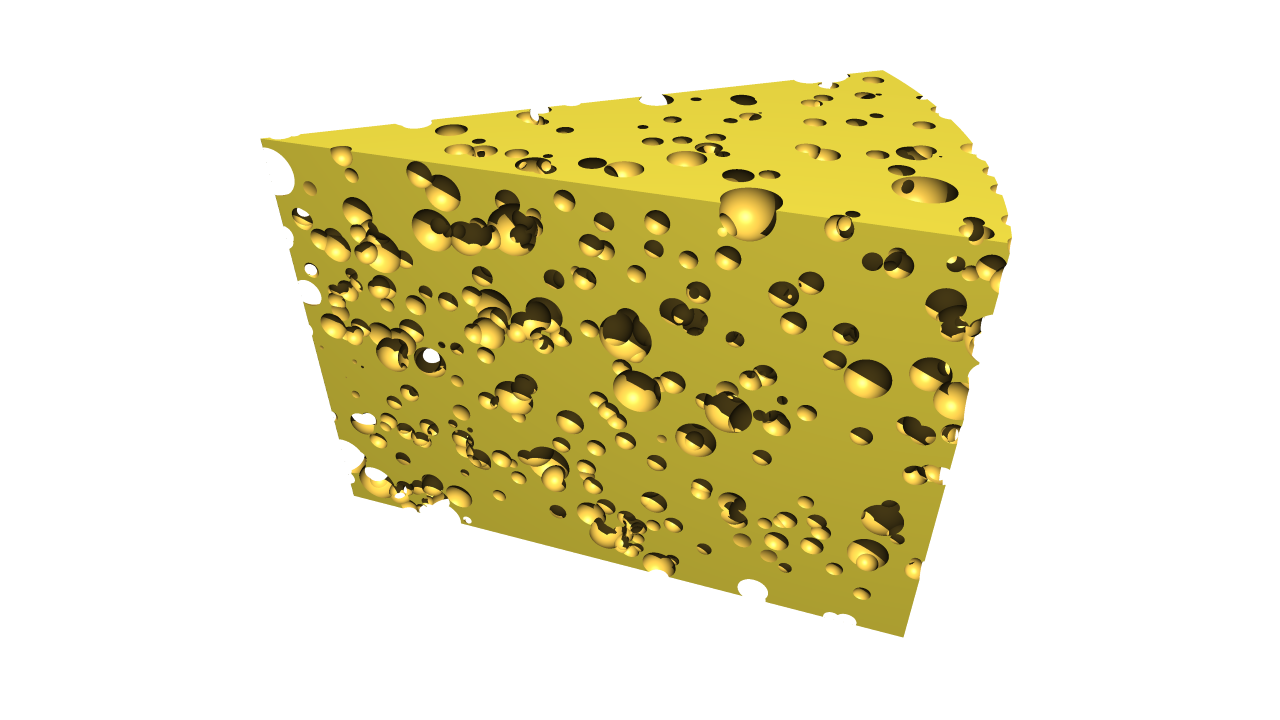
\includegraphics[width=0.95\linewidth]{screenshot_21} \\ б)
  \end{minipage}
  \hfill
  \begin{minipage}[ht]{0.325\linewidth}\centering
    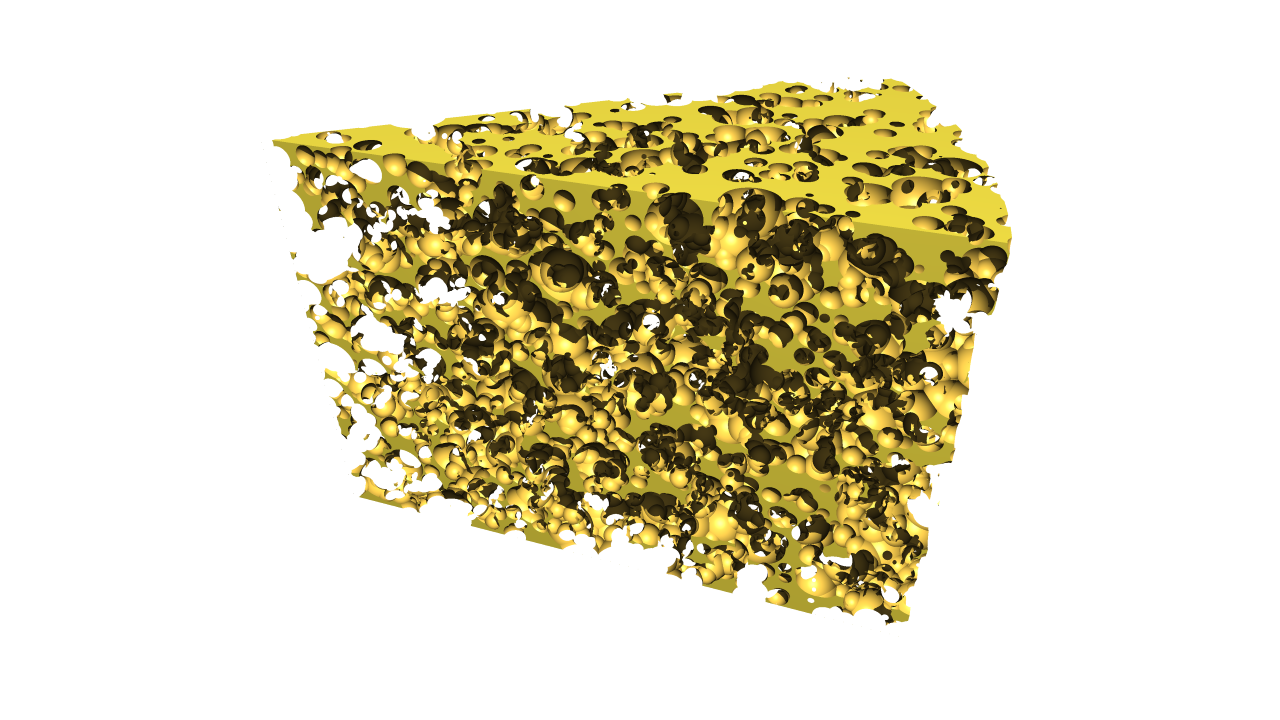
\includegraphics[width=0.95\linewidth]{screenshot_22} \\ в)
  \end{minipage}
  \caption{Сцена «Швейцарский сыр»}
  \label{fig:results_cheese}  
\end{figure}

\begin{figure}[ht]
  \begin{minipage}[ht]{0.325\linewidth}\centering
    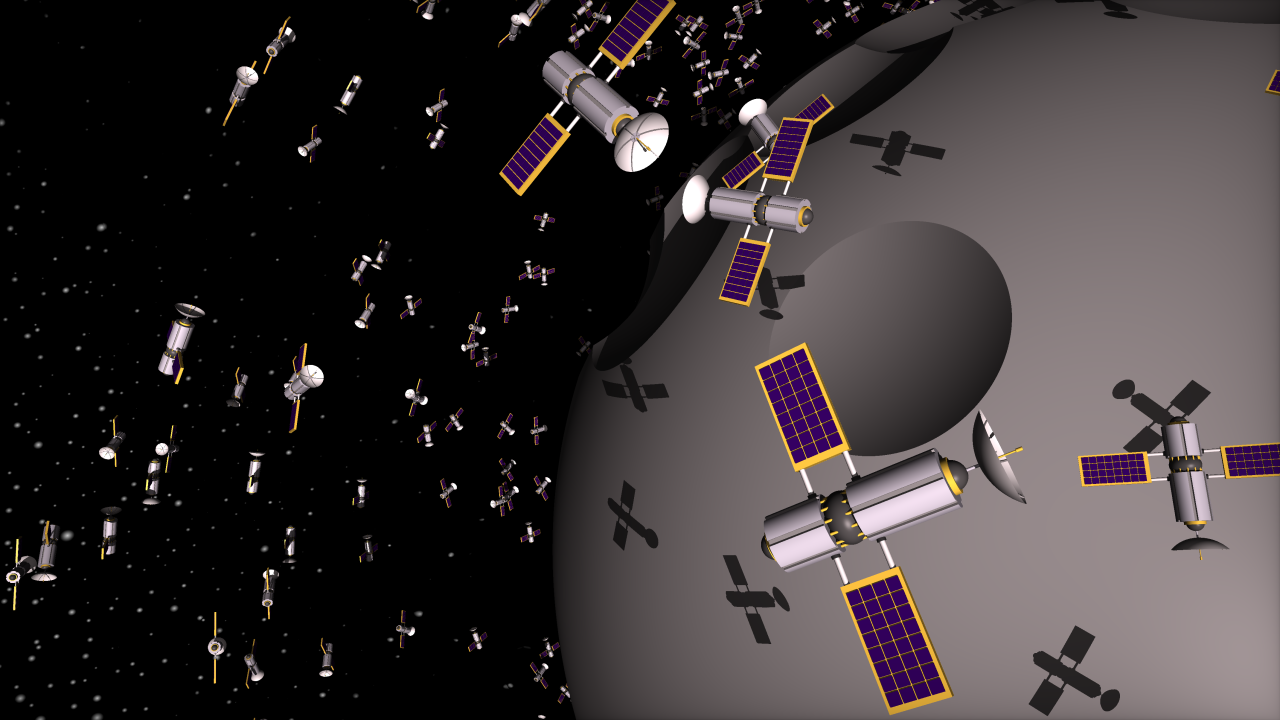
\includegraphics[width=0.95\linewidth]{screenshot_40} \\ а)
  \end{minipage}
  \hfill
  \begin{minipage}[ht]{0.325\linewidth}\centering
    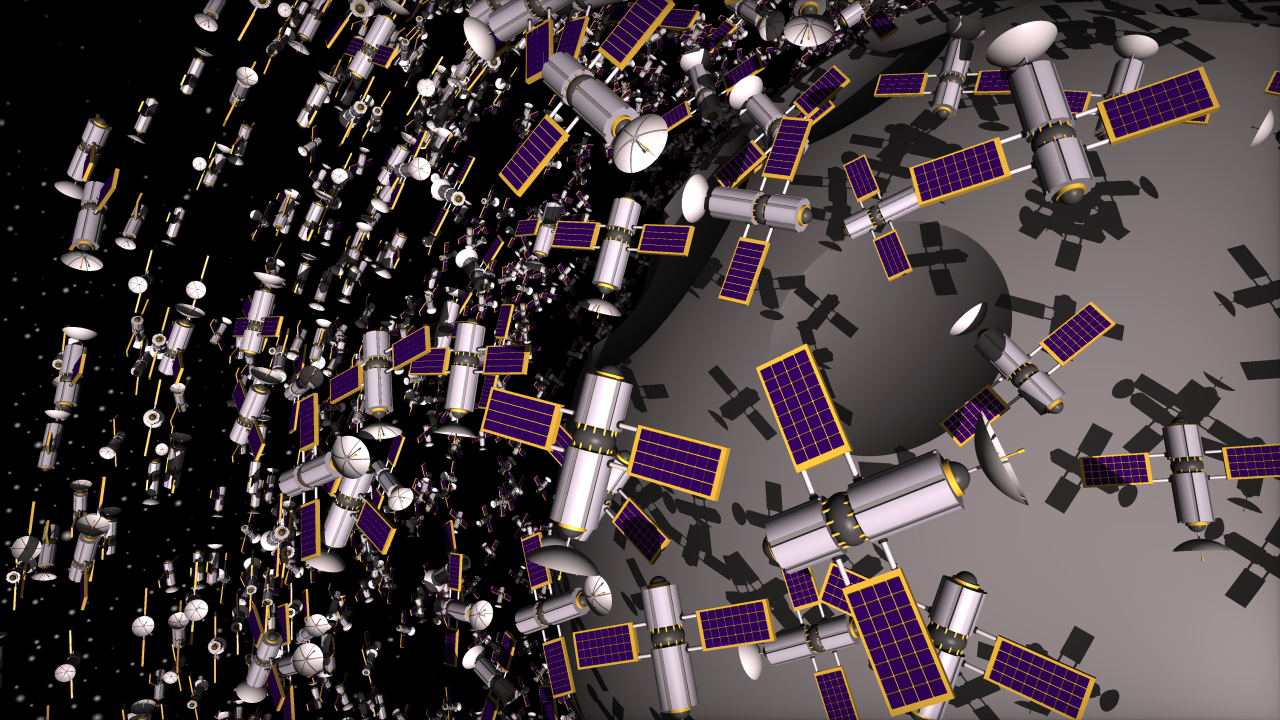
\includegraphics[width=0.95\linewidth]{screenshot_42} \\ б)
  \end{minipage}
  \hfill
  \begin{minipage}[ht]{0.325\linewidth}\centering
    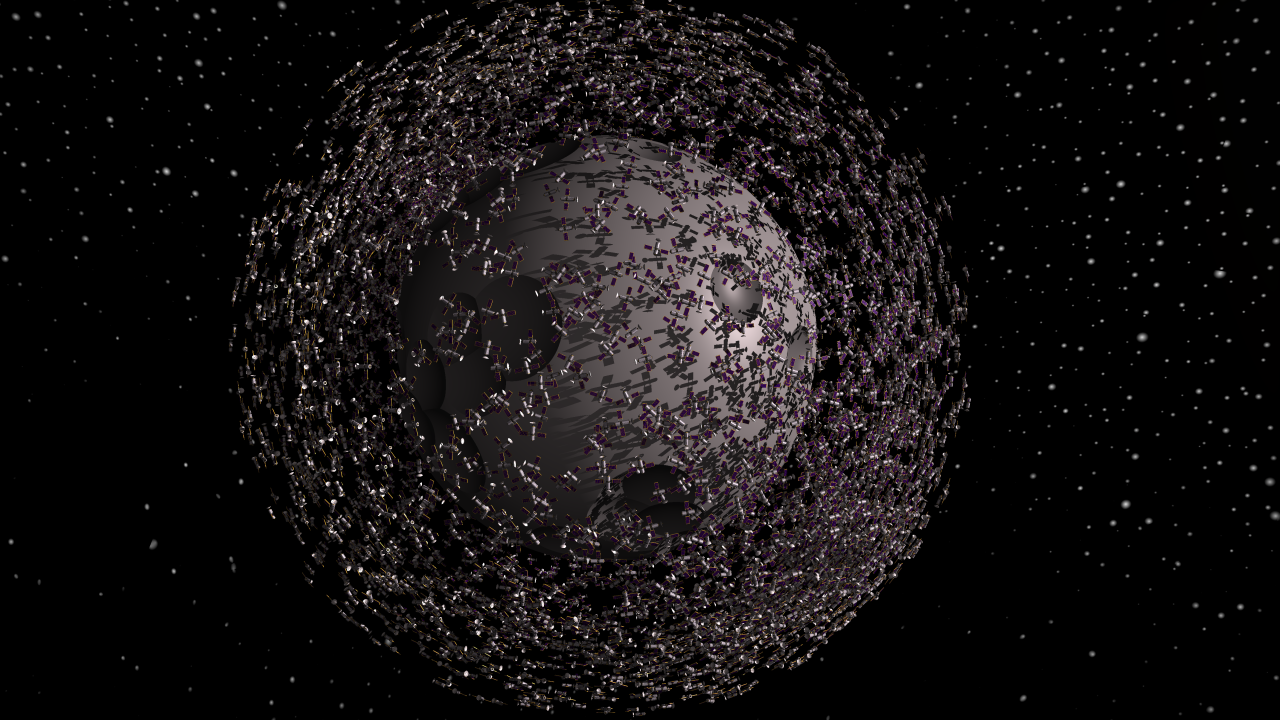
\includegraphics[width=0.95\linewidth]{screenshot_43} \\ в)
  \end{minipage}
  \caption{Сцена «Спутники» (варианты б и в отличаются только ракурсом)}
  \label{fig:results_sat}  
\end{figure}

Третья сцена демонстрирует спутники, вращающиеся вокруг планеты (см. Рисунок \ref{fig:results_sat}). В этой сцене, каждый спутник представлен отдельным CSG деревом. В рамках предложенного решения, набор независимых спутников присутствует в сцене как отдельные узлы BVH дерева верхнего уровня. В таком варианте представления сцены между отдельными спутниками невозможны Булевы операции, однако, так как все CSG деревья независимы, их изменения так-же могут быть независимыми. В то же время, благодаря быстрой процедуре перестроения BVH дерева верхнего уровня, взаимное положение спутников можно изменять динамически (например для анимации или для интерактивного редактирования сцены). Для измерения производительности такого подхода спутники движутся вокруг планеты по случайным круговым траекториям (см. Таблицу \ref{tbl:timings}).

В результате экспериментов, было обнаружено, что производительность предложенного решения линейно масштабируется с ростом тактовой частоты вычислительных ядер графического процессора (см. Рисунок \ref{fig:measurements}). Таким образом, предложенный алгоритм позволяет надеяться на дальнейший рост производительности по мере выхода новых поколений графических чипов. Тактовая частота памяти графического процессора, напротив, не влияет на производительность, что подтверждает предположение, что пропускная способность памяти не является главным ограничивающим фактором для предложенного алгоритма визуализации CSG моделей.

\begin{figure}[ht] 
  \centering
  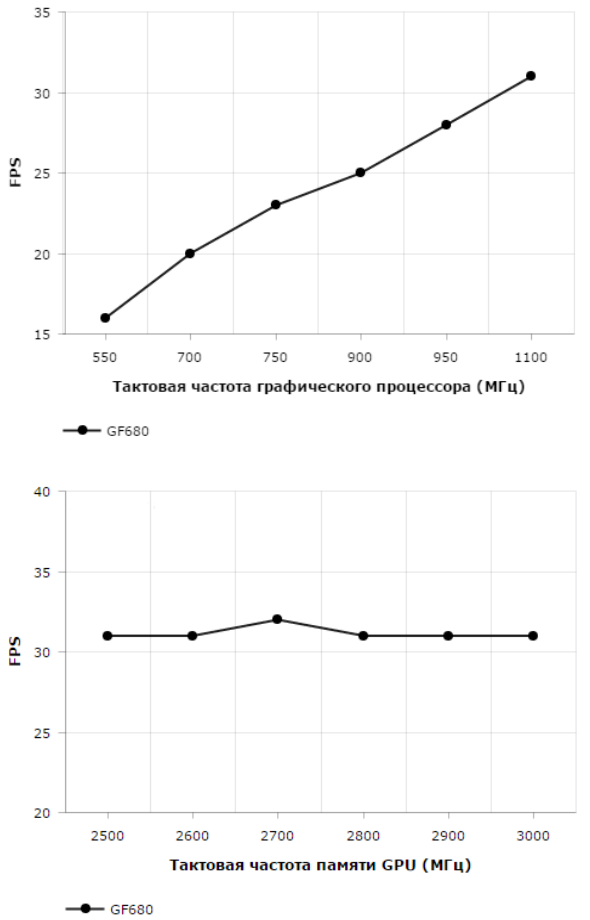
\includegraphics [scale=0.6] {measurements}
  \caption{Производительность на сцене «Швейцарский сыр» в зависимости от тактовой частоты (GF GTX 680)}
  \label{fig:measurements}
\end{figure}

Рассмотрим основные факторы, влияющие на производительность визуализации. Первым фактором, как и для всех методов, основанных на трассировке лучей, является разрешение экрана. Величина FPS меняется практически обратно пропорционально числу обработанных пикселей. Следующий важный фактор - это число примитивов в CSG модели, однако зависимость производительности от данного фактора сложнее. Эксперименты показывают, что, хотя визуализация сцены «Город», содержащей около миллиона CSG примитивов не вызывает затруднений, модель «Швейцарского сыра» показывает совершенно другие результаты. Такую разницу можно объяснить обширными перекрытиями примитивов в модели «Швейцарского сыра», которые заставляют алгоритм многократно проходить по CSG поддеревьям для однозначной классификации точек поверхности. Более того, из-за перекрытия ограничивающих объёмов также падает и эффективность пространственной сортировки узлов. Однако, даже на такой сложной сцене  алгоритм показывает зависимость производительности от числа примитивов близкую к линейной.

Представляет интерес сравнение производительности  GPU-реализации предложенного алгоритма с аналогами. Такое сравнение выполнено на наиболее сложном для алгоритма примере с «сыром» (табл. \ref{tbl:comparison}), в котором производительность аналогов превышена в 5 и более раз.

\begin{table} [htbp]%
    \centering
	\caption{Сравнение производительности (в FPS на GF GTX 680) с решениями-аналогами OpenSG и IceSL \cite{lefebvre2013icesl}}%
	\label{tbl:comparison}
    \renewcommand{\arraystretch}{1.5}
    \begin{SingleSpace}
	\begin{tabular}{@{}@{\extracolsep{20pt}}llll@{}}
        \toprule
    	Сцена	& Предложенное решение & OpenSG	& IceSL	\\
        \midrule 
    	Сыр 1K 	& 128 	 & 2.1		& 1.1		\\
    	Сыр 8K	& 32 	 & 6.5		& 0.3		\\
    	Сыр 32K	& 4 	 & $\sim\!0$ & $\sim\!0$		\\
        \bottomrule
	\end{tabular}%
   	\end{SingleSpace}
\end{table}

Так как предложенное решение основано на трассировке лучей, оно было дополнено для поддержки визуальных эффектов глобального освещения, таких как прозрачность, мягкие тени, отражения, преломления и т.д (рис.~\ref{fig:photorealistic1}, рис.~\ref{fig:photorealistic2}).

\begin{figure}[ht] 
  \centering
  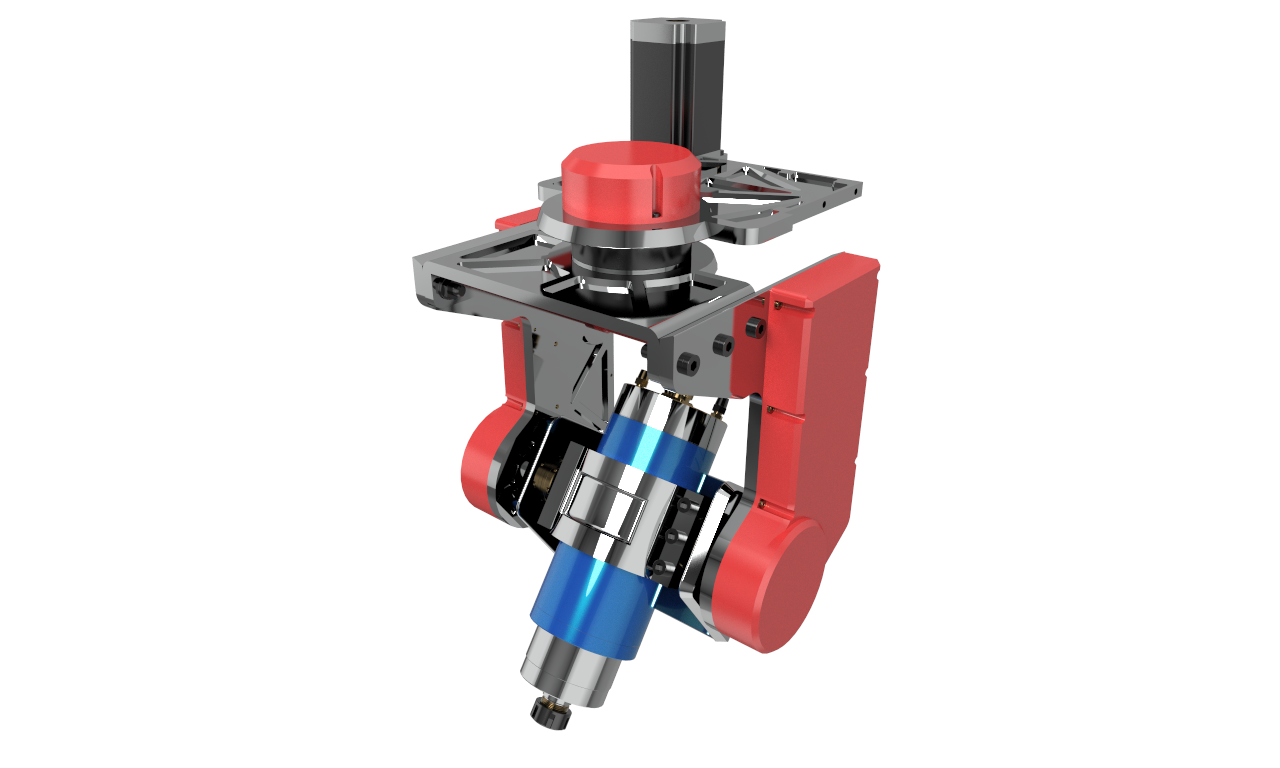
\includegraphics [scale=0.4] {2axis_milling}
  \caption{Фотореалистичная визуализация CSG модели 2-осевой фрезерной головки (построена на основе модели Tamas Cserto)}
  \label{fig:photorealistic1}
\end{figure}

\begin{figure}[ht] 
  \centering
  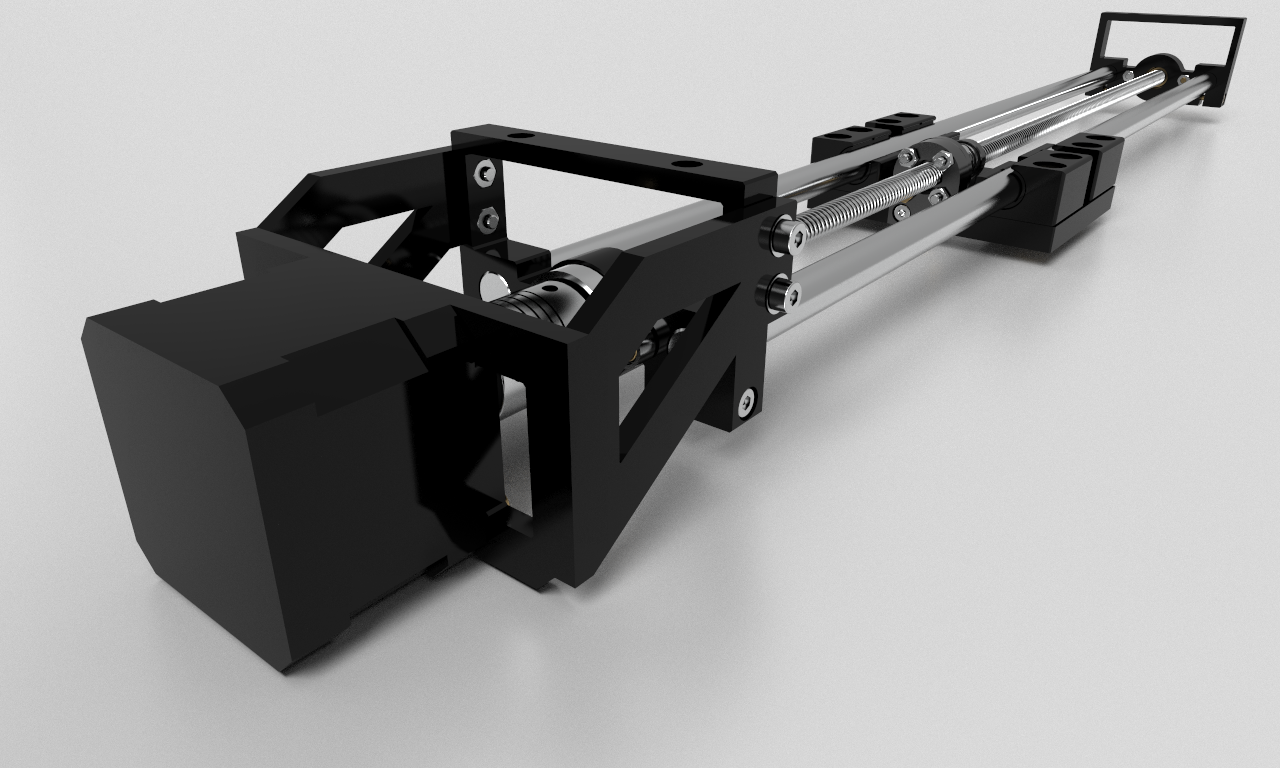
\includegraphics [scale=0.4] {linear_actuator}
  \caption{Фотореалистичная визуализация CSG модели линейного привода (построена на основе модели Aleksej Kolenčenko)}
  \label{fig:photorealistic2}
\end{figure}

Для полноценного включения визуализации CSG-моделей трассировкой лучей в САПР было обеспечено включение результата трассировки в стандартный конвейер растеризации 3D сцен, реализуемый OpenGL/GLSL. С этой целью, используя матрицу проецирования, для каждого луча вычисляется глубина точки пересечения очередного фрагмента, которая затем записывается в буфер глубины OpenGL. В результате визуализация CSG модели может быть дополнена произвольным текстом, линиями осей, сетками либо произвольными триангулированными объектами, отрисованными с помощью OpenGL.           % Глава 3
\chapter*{Заключение}						% Заголовок
\addcontentsline{toc}{chapter}{Заключение}	% Добавляем его в оглавление

Основные результаты работы заключаются в следующем:

\begin{enumerate}
  \item Предложен, реализован и экспериментально исследован алгоритм трассировки лучей, предназначенный для высокопроизводительной фотореалистичной визуализации в полноэкранном разрешении очень больших и структурно сложных сцен (до 1 миллиона примитивов, при глубине CSG дерева до 24), выполненных в конструктивном представлении (CSG). Задачи визуализации такой сложности возникают в CAD-системах в процессе проектирования высокотехнологичных технических объектов и крупных промышленных производств. В отличие от аналогов, алгоритм рассчитывает изображение за один проход и не накладывает ограничений на число примитивов и глубину дерева их структуры, позволяет получать точный результат без предварительной тесселяции CSG-сцены. Наивысшая производительность алгоритма достигается на GPU. Для технической визуализации достигается режим  реального времени, для фотореалистичной "--- режим интерактивного взаимодействия. В качестве примитивов могут использоваться классические формы и объекты, определяемые аналитически (в частности, поверхности второго порядка или неявно заданные функции). Число примитивов ограничено только доступной графической памятью, в то время как производительность линейно масштабируется с ростом числа и тактовой частоты вычислительных ядер.

  \item Оптимизированы для GPU структуры данных и производительность процедуры MIS (multiple impotance sampling), важнейшей для производительности и качества результата методов глобального освещения.

  \item В известный Kensler's CSG ray-tracing алгоритм (2006), введен высокоуровневый автомат со стековой памятью, управляющий алгоритмом Kensler-а, в результате чего построен итеративный алгоритм трассировки CSG адаптированный для GPU.

  \item Предложен и реализован метод оптимизации CSG моделей, преобразующий входное дерево в пространственно-отсортированную форму близкую к сбалансированной. После оптимизации производительность визуализации зависит только от вычислительных возможностей GPU (в отличии от аналогов не имеет ограниченния пропускной способностью памяти).

  \item Найдено оригинальное решение, обеспечивающее возможность глубокой оптимизации CSG дерева. Оптимизация декомпозирована на 4 шага: а) преобразование CSG-выражения в позитивную форму (представление только коммутативными операциями, разрешившее пространственную оптимизацию); б) пространственная оптимизация (со сборкой однородных операций в блоки); в)оптимизация высоты (балансировка) дерева; г) преобразование в исходную форму.

  \item Разработано экспериментальное программное обеспечение способное на порядок увеличить производительность синтеза изображений сложных CSG-моделей в САПР и сделать процесс работы с проектами сложных технических комплексов и промышленных предприятий процессом реального времени.

\end{enumerate}


После рассмотренной серии публикаций по созданию высокопроизводительных алгоритмов и библиотек CSG-визуализации, начиная с создания открытой библиотеки OpenSG \todo{ours[11]} и закрывая список работой \todo{[7]}, казалось, что вопрос о высокопроизводительной визуализации сложных CSG-сцен удовлетворительно решен. Но, тем не менее, практика современного проектирования вновь ставит этот вопрос на повестку дня. Достигнутый результат существенно продвинул прежнее представление о трассировке сложных CSG-сцен. Планируется продолжить исследование и развитие предложенного алгоритма.
      % Заключение
%\include{Dissertation/acronyms}        % Список сокращений и условных обозначений
%\include{Dissertation/dictionary}      % Словарь терминов
\include{Dissertation/references}      % Список литературы
\include{Dissertation/lists}           % Списки таблиц и изображений (иллюстративный материал)
% \include{Dissertation/appendix}        % Приложения

\end{document}
